%=================================================
%=================================================
%
% WARNING: NOT USED IN opal_user_guide.tex
%
%=================================================
%=================================================

\ifdefined \buildingFullOPALManual \else


%\ifx \@buildingFullOPALManual \@empty
%\else

%\documentclass[12pt,a4paper]{report}
\documentclass[a4paper]{book}

%% does not work in Latex2Html mode
%\usepackage{hyperref}

\usepackage[T1]{fontenc}
\usepackage{url}
\usepackage{html}
\usepackage{epic}
\usepackage{eepic}
\usepackage{makeidx}
\usepackage{array}
\usepackage{times}
\usepackage{amsmath}
\usepackage{amsxtra}
\usepackage{bm}
\usepackage[thin,thinp,thinc]{esdiff}
\usepackage{graphicx}
\usepackage{dingbat}
\usepackage{color}
\usepackage{subfig}
\usepackage{boxedminipage}
\usepackage{alltt}
\usepackage{nicefrac}
\usepackage{calc}
%\usepackage{pdfdraftcopy}             % Draft
\usepackage{tikz}
\usetikzlibrary{
  er,3d,calc,fadings,trees,positioning,arrows,chains,decorations.pathreplacing,
  decorations.pathmorphing,shapes,shapes.symbols,shapes.arrows,matrix,through,decorations.text
}

\tikzset{
  >=stealth',
  punktchain/.style={rectangle,rounded corners, draw=black, very thick,text width=10em,
                     minimum height=3em, text centered, on chain},
  line/.style={draw, thick, <-},
  element/.style={tape,top color=white,bottom color=blue!50!black!60!,minimum width=8em,
                  draw=blue!40!black!90, very thick,text width=10em, minimum height=3.5em,
                  text centered, on chain},
  every join/.style={->, thick,shorten >=1pt},
  tuborg/.style={decorate},
  tubnode/.style={midway, right=2pt}
}

\tikzstyle{material}=[draw, fill=blue!20, text width=16.0em, text centered, minimum height=1.5em]
\tikzstyle{diagramstep} = [material, text width=20em, minimum width=10em, minimum height=3em, rounded corners]
\tikzstyle{line} = [draw, thick, color=black!50, -latex']

\usepackage{booktabs}
\usepackage{xspace}
\usepackage{xstring}

\usepackage{fancyvrb}
\usepackage{rotating}
\usepackage{float}

\usepackage{tabularx}
\usepackage{longtable}
\setcounter{LTchunksize}{3}

\usepackage[section]{placeins}
\usepackage{MnSymbol}
\usepackage{microtype}
\usepackage{setspace}
\usepackage{dcolumn}

\usepackage[vmargin={3.0cm,3.0cm},
            hmargin={2.0cm,3.0cm}]{geometry}

\usepackage{upgreek}
\usepackage[binary-units=true]{siunitx}
\sisetup{exponent-product = \cdot,math-ohm=\Upomega,text-ohm=\ensuremath{\Upomega}}
\DeclareSIUnit{\clight}{c}
\DeclareSIUnit\gauss{Ga}

\usepackage{engord}
\usepackage{wasysym}
\DeclareSIUnit[number-unit-product = \,]{\permill}{\permil}

\usepackage{hyperref}
\hypersetup{
    pdftitle          = The OPAL Framework,
    pdfauthor         = {Andreas Adelmann, Achim Gsell, Valeria Rizzoglio, Christof Metzger-Kraus,
                         Yves Ineichen, Xiaoying Pang, Steve Russell, Chuan Wang, Jianjun Yang,
                         Suzanne Sheehy, Chris Rogers, Daniel Winklehner},
    pdfsubject        = User's Reference Manual,
    pdffitwindow      = true,               % page fit to window when opened
    pdfnewwindow      = true,               % links in new window
    colorlinks        = true,               % false: boxed links; true: colored links
    linkcolor         = black!80!green,     % color of internal links
    citecolor         = black!20!red,       % color of links to bibliography
    urlcolor          = blue,               % color of external links
    breaklinks        = true,
    bookmarksnumbered = true,
    plainpages        = false
}

\usepackage{ifthen}

\newif \iflinuxwindows
\linuxwindowstrue   % set this to true when building the manual on Linux or Windows
\iflinuxwindows
\usepackage{epstopdf}
\fi

\usepackage[backend=biber,
            style=phys,
            biblabel=brackets,
            maxnames=3,
            doi=true,
            isbn=true,
            url=true]{biblatex}
%---- macros ----

\renewcommand{\topfraction}{1.0}
\renewcommand{\bottomfraction}{1.0}
\renewcommand{\textfraction}{0.0}
\renewcommand{\arraystretch}{2.0}
\newenvironment{tex2html_nowrap}{}{}


\newcommand{\Newline}{\hfil \\}


\newsavebox{\ExampleBox}
\newenvironment{example}
 {\VerbatimEnvironment
  \begin{flushleft}
  \begin{lrbox}{\ExampleBox}
    \begin{minipage}{\linewidth}
  \begin{Verbatim}[frame=lines,xleftmargin=0cm,fontsize=\footnotesize,samepage=true]}
 {\end{Verbatim}
  \end{minipage}
  \end{lrbox}
  \mbox{\usebox{\ExampleBox}}
  \end{flushleft}
 }

\newenvironment{longexample}
{\Verbatim[frame=lines,xleftmargin=0mm,fontsize=\footnotesize]}
{\endVerbatim}

%\examplefromfile{filename} reads in a text file and displays it in the document.
\newcommand{\examplefromfile}[1]{
\VerbatimInput[frame=lines,xleftmargin=0mm,fontsize=\footnotesize,label=\texttt{#1}]{#1}}

%for upright d of differentials
\makeatletter
\newcount\my@repeat@count

\newcommand{\myrepeat}[2]{%
  \begingroup
  \my@repeat@count=\z@
  \@whilenum\my@repeat@count<#1\do{#2\advance\my@repeat@count\@ne}%
  \endgroup
}

\newcommand{\differential}[1]{\ifstrempty{#1}{\ES@dop\ES@difint}{\ES@dop^{#1}\ES@difint}}
\newcommand{\pdifferential}[1]{\ifstrempty{#1}{{\partial\,}}{{\partial^{#1}\,}}}

\makeatother

\newcommand{\der}[3][]{\frac{\differential{#1}#2}{\differential{}\ifstrempty{#1}{#3}{#3^#1}}}
\newcommand{\parder}[3][]{\frac{\pdifferential{#1}#2}{\pdifferential{}\ifstrempty{#1}{#3}{#3^#1}}}
\newcommand{\niceder}[3][]{\nicefrac{\differential{#1}#2}{\differential{}\ifstrempty{#1}{#3}{#3^#1}}}
\newcommand{\uglyder}[3][]{{\differential{#1}#2}/{\differential{}\ifstrempty{#1}{#3}{#3^#1}}}
\newcommand{\uglyparder}[3][]{{\pdifferential{#1}#2}/{\pdifferential{}\ifstrempty{#1}{#3}{#3^#1}}}
\newcommand{\dd}[1][]{\; \differential{#1}}
\newcommand{\primed}{^{\prime}}
\newcommand{\dprimed}{^{\prime\prime}}
\newcommand{\nprimed}[1]{^{\myrepeat{#1}{\prime}}}

%Editing Macros
\newcommand{\TODO}[1]{{\color{red}\ifthenelse{\boolean{ShowDebug}}{[TODO: #1]}{}}}



%text in gray box
\newsavebox{\fmbox}
\definecolor{lightgray}{gray}{0.95}
\newenvironment{fmpage}
   {\vspace{-1.0cm}\begin{lrbox}{\fmbox}\begin{minipage}[t]{13.5cm}\vspace{0.1cm}}
   {\vspace{-0.4cm}\end{minipage}\end{lrbox}\begin{center}\fcolorbox{black}{lightgray}{\usebox{\fmbox}}\end{center}}


% Definition new signes
\newcommand{\R}{{\mathbb R}} % real numbers
\newcommand{\Q}{{\mathbb Q}} % rational numbers
\newcommand{\Z}{{\mathbb Z}} % integer numbers
\newcommand{\N}{{\mathbb N}} % natural numbers

\newcommand{\mad}{\textsc{mad}\xspace}
\newcommand{\madnine}{\textsc{mad9}\xspace}
\newcommand{\madninep}{\textsc{mad9p}\xspace}
\newcommand{\madeight}{\textsc{mad8}\xspace}
\newcommand{\classic}{\textsc{classic}\xspace}

\makeatletter
\newcommand{\opal@impl}{\textsc{Opal}}
\newcommand{\opalt@impl}{\textsc{Opal-t}}
\newcommand{\opalcycl@impl}{\textsc{Opal-cycl}}
\newcommand{\opalmap@impl}{\textsc{Opal-map}}
\newcommand{\opalenv@impl}{\textsc{Opal-e}}

\newcommand{\opal}{\opal@impl\xspace}
\newcommand{\opalt}{\opalt@impl\xspace}
\newcommand{\opalcycl}{\opalcycl@impl\xspace}
\newcommand{\opalmap}{\opalmap@impl\xspace}
\newcommand{\opalenv}{\opalenv@impl\xspace}

\newcommand{\noopalt}{\leftthumbsdown \opalt@impl\xspace}
\newcommand{\noopalcycl}{\leftthumbsdown \opalcycl@impl\xspace}
\newcommand{\noopalmap}{\leftthumbsdown \opalmap@impl\xspace}
\newcommand{\noopalenv}{\leftthumbsdown \opalenv@impl\xspace}
\makeatother

\newcommand{\impactt}{\textsc{Impact-t}\xspace}
\newcommand{\partroot}{\textsc{H5root}}


\newcommand{\latermore}{More details will be given in Version 1.6.0}


\newcommand{\lieop}[1]{{:}{#1}{:}}

\newcommand{\rms}[1]{\overset{\sim}{#1}}

\newcommand{\sprod}{\cdot}
\newcommand{\vprod}{\times}
\newcommand{\matr}[1]{\mathcal{#1}}
\renewcommand{\vec}[1]{{\bm{#1}}}
\newcommand{\transpose}[1]{#1^\intercal}
\renewcommand{\epsilon}{\varepsilon}

\newcommand{\keyword}[2][]{\ifstrempty{#1}{\texttt{\expandafter\MakeUppercase\expandafter{#2}}}{\hyperref[#1]{\texttt{\expandafter\MakeUppercase\expandafter{#2}}}}}
\newcommand{\tabline}[3][]{\keyword[#1]{#2}& #3 \\}
\newcommand{\tabheadcell}[1]{{\bfseries #1}}

\newcommand*\kdescriptionlabel[1]{\hspace\labelsep
                                \normalfont\keyword{#1}\index{#1}}
\makeatletter
\newenvironment{kdescription}
               {\list{}{\labelwidth\z@ \itemindent-\leftmargin
                        \let\makelabel\kdescriptionlabel}}
               {\endlist}
\makeatother

\ExplSyntaxOn
\NewDocumentCommand{\tabhead}{ m }
 {
  \seq_set_split:Nnn \l_tmpa_seq { & } { #1 }
  \bfseries \seq_use:Nn \l_tmpa_seq { & \bfseries } \\
 }

\NewDocumentCommand \multrefImpl { O{ } m m m } {
  \ifnumgreater{\clist_count:n {#4}}{1}{
    \seq_set_from_clist:Nn \l_tmpa_seq { #4 }

    \seq_set_map:NNn \l_tmpb_seq \l_tmpa_seq { \exp_not:n { \ref{#3:##1} } }
    \ifstrempty{#1}{#2s}{#1}~\seq_use:Nnnn \l_tmpb_seq {\ and\ } {,\ } {,\ and\ }
  }{
    #2~\ref{#3:#4}
  }
}

\NewDocumentCommand \multeqnrefImpl { m } {
  \ifnumgreater{\clist_count:n {#1}}{1}{
    \seq_set_from_clist:Nn \l_tmpa_seq { #1 }

    \seq_set_map:NNn \l_tmpb_seq \l_tmpa_seq { \exp_not:n { \eqref{eq:##1} } }
    Equations~\seq_use:Nnnn \l_tmpb_seq {\ and\ } {,\ } {,\ and\ }
  }{
    Equation~\eqref{eq:#1}
  }
}
\ExplSyntaxOff


%Abbreviations for Equations, Figures, and Tables
%\newcommand{\Equation}[1]{Equation~\eqref{#1}}

\newcommand{\bibref}[2]{#1 \cite{bib:#2}}
\newcommand{\figref}[1]{\multrefImpl{Figure}{fig}{#1}}
\newcommand{\chpref}[1]{\multrefImpl{Chapter}{chp}{#1}}
\newcommand{\appref}[1]{\multrefImpl[Appendices]{Appendix}{chp}{#1}}
\newcommand{\secref}[1]{\multrefImpl{Section}{sec}{#1}}
\newcommand{\ssecref}[1]{\multrefImpl{Section}{ssec}{#1}}
\newcommand{\tabref}[1]{\multrefImpl{Table}{tab}{#1}}
\newcommand{\eqnref}[1]{\multeqnrefImpl{#1}}

\newcommand{\seefig}[1]{(see~\figref{#1})}
\newcommand{\seechp}[1]{(see~\chpref{#1})}
\newcommand{\seesec}[1]{(see~\secref{#1})}
\newcommand{\seessec}[1]{(see~\ssecref{#1})}
\newcommand{\seetab}[1]{(see~\tabref{#1})}
\newcommand{\seeeqn}[1]{(see~\eqnref{#1})}

\newcommand{\filename}[1]{\emph{#1}}


% Define distances for bordering
\newcommand{\blockdist}{1.3}
\newcommand{\edgedist}{1.5}
\newcommand{\diagramstep}[2]{node (p#1) [diagramstep] {#2}}


% place chapter title page on odd pages
\let\stdchapter\chapter
\makeatletter
\renewcommand*{\chapter}{\if@openright\cleardoublepage\else\clearpage\fi\stdchapter}

\makeatother

\IfFileExists{./version.tex}{%
  \newcommand{\opalversion}[1]{Version \ifstrempty{#1}{1.9.0}{#1}\xspace}
%
}%
{%
  \newcommand{\opalversion}[1]{\ifstrempty{#1}{current Version}{Version #1}\xspace}%
}
\newboolean{ShowMap}
\setboolean{ShowMap}{false}

\newboolean{ShowEnv}
\setboolean{ShowEnv}{false}

\newboolean{ShowDebug}
\setboolean{ShowDebug}{false}

%----Control Structures
\newboolean{FullOPALManual}
\setboolean{FullOPALManual}{false}


\makeindex


\bibliography{bibliography}
\begin{document}

\fi


\chapter{\opal Flavours}
\label{chp:opalFlavours}
\index{opalFlavours}

\section{\opalt}
\opalt is a fully three-dimensional program to track in time, relativistic particles taking into account space charge forces, self-consistently in the electrostatic approximation, and short-range longitudinal and transverse wake fields. \opalt is one of the few
codes  that is implemented using a parallel programming paradigm from the ground up. This makes \opalt indispensable for
high statistics simulations of various kinds of existing and new accelerators. It has a comprehensive set of beamline
elements, and furthermore allows arbitrary overlap of their fields, which gives \opalt a capability
to model both the standing wave structure and traveling wave structure. Beside IMPACT-T it is the only code making use of
space charge solvers based on an integrated Green \cite{qiang2005, qiang2006-1,qiang2006-2} function to efficiently and accurately treat beams with
large aspect ratio, and a shifted Green function to efficiently treat image charge effects of a cathode \cite{fubiani2006,qiang2006-1,qiang2006-2}.
For simulations of particles sources i.e. electron guns \opalt uses the technique of  energy binning in the electrostatic space charge calculation to model beams with large
energy spread. In the very near future a parallel Multi Grid solver taking into account the exact geometry will be implemented.

\subsection{Integration of the Equation of Motion}
\opalt integrates the relativistic Lorentz equation
\begin{equation}
F(\vec{x},\vec{v},t) = m_0 \frac{\gamma \vec{v}}{dt} =   \frac{q}{m}[\vec{E}_{ext} + \vec{E}_{sc} + \vec{v} \times (\vec{B}_{ext} + \vec{B}_{sc})]
\end{equation}
where $\gamma$ is the relativistic mass factor and $\vec{E}$  and $\vec{B}$ are abbreviations for $\vec{E}(\vec{x},\vec{v},t)$ and $\vec{B}(\vec{x},\vec{v},t)$
respectively. \latermore .

%    NEED WORK ADA
%\begin{equation}
%\vec{x}_{n+1/2} = \vec{x}_{n} + \frac{1}{2}\vec{v}_{n-1/2}\quad (= \vec{x}_{n} + \frac{\Delta t}{2} \frac{\vec{\beta}_{n-1/2}\gamma_{n-1/2}}{\gamma_{n-1/2}})
%\end{equation}

%Update the momenta using the $D_1$ algorithm as described in Birdsall and Langdon's book.

%\begin{equation}
%    \vec{v}_{n+1/2} = \frac{1}{2} \overline{\vec{a}_{n}}   \Delta t +  R \cdot (\vec{v}_{n-1/2} + \frac{1}{2} \overline{\vec{a}_{n}}  \Delta t)
%\end{equation}
%
%
%         where the operator $R$ effects a rotation through angle $-2\tan^{-1}(\vec{\Omega} \Delta t/2)$ where $\vec{\Omega} = Q \vec{B}_{n}/(m_{e} c)$.
%        $R$ can be written as
%        \begin{equation}
%         R = \frac{(1 - \Theta^2) I + 2  \Theta \transpose{\Theta} - 2  \Theta \times I }{1+\Theta}
%        \end{equation}
%        where $\vec{\Theta} = \vec{\Omega}  \Delta t/2 $ and $I$ is the unit tensor.
%


\subsection{Space Charge}
\label{sec:opalFlavours:spacecharge}
\index{SpaceCharge}
space charge effects will be included in the simulation by specifying a field solver described in \chpref{fieldsolver} and using the solver in the
track command described in \chpref{track}.
By default, the code does not assume any symmetry i.e. full 3D. In the near future it is planed to implement also a slice (2D) model.
This will allow the use of less numbers of macro-particles in the simulation which reduces the computational time
significantly.

The space charge forces are calculated by solving the 3D Poisson equation with open boundary conditions
using a standard or integrated Green function method. The image charge effects of the conducting cathode are also
included using a shifted Green function method. If more than one Lorentz frame is defined, the total space charge forces are then the summation of contributions from all Lorentz frames. \latermore

\subsubsection{FFT Based Particle-Mesh (PM) Solver}
 \latermore

%    NEED WORK ADA
%The Particle-Mesh (PM) \cite{hockney} solver is one of the oldest improvements over the PP solver. Still one of the best references is the book by R.W.~Hockney \& J.W.~Eastwood \cite{hockney}.
%The PM solver introduces a discretization of space. The rectangular computation domain $\Omega:=[-L_x,L_x]\times[-L_y,L_y]\times[-L_t,L_t]$, just big enough to include all particles, is segmented into a regular mesh of $M=M_x\times M_y\times M_t$ grid points.


%In order to obtain  ${\cal M}_2$ in \Eq{eq:splitOper1} we must solve Poisson's equation,
%where $\rho$ stands for the
%charge density and $\phi$ for the scalar electrostatic potential:
%\begin{equation}\label{Poisson}
%\nabla^2 \phi(\vec{q}) = - \frac{\rho(\vec{q})}{\epsilon_0}
%\end{equation}
%subject to open boundary conditions in all spatial directions: $\phi (\vec{q}) \rightarrow 0$ as $|\vec{q}| \rightarrow \infty$ or
%imposing periodic boundary conditions in longitudinal directions. The assumption of using an ``isolated system`` is physically
%motivated by observing the ratio of the beam size to vacuum vessel domensions. It has the computational advantages that one can use cyclic convolution in \eqref{eq:FourierPoisson}.
%The computational domain $\Omega \subset \R^3$ is simply connected and has a cylindrical
%or rectilinear shape.
%The corresponding integral equation reads:
%\begin{equation}
%\phi(\vec{q}) = \dis\int\limits_\Omega \, G(\vec{q} - \vec{q}\primed) \,\rho (\vec{q'}) \,d \vec{q}\primed , \;\;\Omega \subset \R^3
%\end{equation}
%where $G$ is the Green's function which gives the response to a unit source term. In 3D we have
%\begin{equation}
%G(\vec{q}-\vec{q}\primed) = \dis\frac{1}{4 \pi \,|\vec{q} - \vec{q}\primed|} \,.
%\end{equation}
%The electric field then follows from the electrostatic potential
%\begin{equation}\label{Electric}
%\vec{E} = - \nabla \phi.
%\end{equation}

%The charges are assigned from the particle positions in continuum, onto the grid using
%one of two available interpolation schemes: cloud in cell (CIC) or nearest grid point (NGP).
%Then the Poisson equation is solved on the mesh and the electric field at the particle positions is obtained by
%interpolating back from the mesh. The use of the convolution theorem to solve the discretized Poisson
%equation \eqref{Poisson} on the grid can dramatically improve performance.

%Let $\Omega^D$ be spanned by a mesh of $l \times n \times m$ with $l= 1 \dots M_x$, $n= 1\dots M_x$ and $m= 1 \dots M_t$.
%The solution of the discretized Poisson equation with $\vec{k}=(l,n,m,)$
%\begin{equation}\label{eq:DiscretizedPoisson}
%\nabla^{2} \phi^D(\vec{k}) = - \frac{\rho^D(\vec{k})}{\epsilon_0}, \vec{k} \in \Omega^D.
%\end{equation}
%$\phi^D$ then is given by convolution with the appropriate discretized Green's function $G_D$:
%\begin{equation}
%\phi^D = \rho^D * G^D.
%\end{equation}
%In Fourier space (hats) the convolution becomes a simple multiplication, with
%\[
%G(\vec{q})=\frac{1}{4\pi}\frac{1}{|\vec{q}|}\longrightarrow  \widehat{G}(\vec{k})=-\frac{1}{4\pi}\frac{1}{|\vec{k}|^2}
%\]
%and we get:
%\begin{equation}\label{eq:FourierPoisson}
%\widehat{\phi}^D = \widehat{\rho}^D \cdot \widehat{G}^D.
%\end{equation}
%Thus, the convolution sum is converted to a single multiplication at the cost of a Fourier transform. Fortunately, Fast Fourier Transform (FFT) on the mesh is a very fast and accurate method
%of transforming mesh-defined quantities to Fourier space. It needs $\mathcal{O}$($M\log M$) computational effort, so that, together with the interpolations, an overall scaling of $\mathcal{O}$($N+M\log M$) is achieved.

%In order to have good spatial resolution, small grid sizes are often necessary, which again require a
%large number of particles. Therefore, both the grid size $M$ and the particle number $N$
%are limiting factors.
%The PM Solver Algorithm is summarized in the following algorithm:
%\begin{tabbing}
%{\bf PM Solver Algorithm}\\
%\quad $\triangleright$ Assign particle charges $q_i$ to nearby mesh points to obtain $\rho^D$ \\
%\quad $\triangleright$ Use FFT on $\rho^D$ and $G^D$ to obtain $\widehat{\rho}^D$ and $\widehat{G}^D$ \\
%\quad $\triangleright$ Determine $\widehat{\phi}^D$ on the grid using $\widehat{\phi}^D = \widehat{\rho}^D \cdot \widehat{G}^D$ \\
%\quad $\triangleright$ Use inverse FFT on $\widehat{\phi }^D$ to obtain $\phi^D$ \\
%\quad $\triangleright$ Compute $\vec{E}^D= -\nabla \phi^D$\footnote{using a second order finite difference method} \\
%\quad $\triangleright$ Interpolate $\vec{E(\vec{q})}$ at particle positions $\vec{q}$ from $\vec{E}^D$  \\
%\end{tabbing}
%\subsubsection{Open and Periodic Boundary Conditions}
%In order to meet open boundary conditions and to remove the intrinsic periodicity of the FFT, the grid size needs to be doubled in all spatial dimensions and the charge distribution is located at only one octant. The charge distribution is set equal to zero elsewhere. If the potential is then calculated in the entire enlarged region, the correct potential for an isolated system is obtained in the `physical' octant. This is referred to as the `Hockney Trick' \cite{hockney}. For periodic boundary conditions in the longitudinal direction, the Hockney trick is applied to the transverse directions only.
%The main drawback of this method is its high storage requirement. However, using symmetries one is
%able to bound the required storage to $2N_g$ where $N_g$ is the grid size used in the physical
%region of the calculation (see \cite{hockney} on p. 213).
\subsubsection{Interpolation Schemes}
 \latermore

%\label{sec:interpol}
%Both charge assignment and electric field interpolation are related to the interpolation
%scheme used. A detailed discussion is given in~\cite{hockney}.
%If $e_i$ is the charge of a particle, we can write the density at mesh point $\vec{k}_m$ as
%\begin{equation}\label{eq:discRho}
%\rho(\vec{k}_m)^D = \sum_{i=1}^N e_i\cdot W(\vec{q}_i,\vec{k}_m), ~ m=1\dots M
%\end{equation}
%where $W$ is a suitably chosen weighting function (with local support).
%The simplest scheme is the nearest grid point (NGP) method, where the total particle charge is assigned to
%the nearest grid point and the electric field is also evaluated at the nearest grid point. A more
%elaborate scheme is called cloud in cell (CIC). It assigns the charge to the $2^d$ nearest grid points and
%also interpolates the electric field from these grid points. The assigned density changes are continuous when
%a particle moves across a cell boundary, although the first derivative is discontinuous. A schematic of the
%CIC interpolation scheme is shown in \figref{CIC} for the two-dimensional case.
%%total momentum consered. errors small at large particle separations. charge assignement schould vary smoothly as particle position changes.
% \begin{figure}
% \begin{center}
%% \includegraphics[width=0.75\linewidth]{\figdir/cic.eps}
% \caption[CIC interpolation scheme]{\label{fig:CIC} \it CIC interpolation scheme.}
% \end{center}
% \end{figure}

\subsubsection{Iterative Space Charge Solver}
This is a scalable parallel solver for the Poisson equation
  within a Particle-In-Cell (PIC) code for the simulation of electron
  beams in particle accelerators of irregular shape.  The problem is
  discretized by Finite Differences.  Depending on the treatment of the
  Dirichlet boundary the resulting system of equations is symmetric or
  `mildly' nonsymmetric positive definite.  In all cases, the system is
  solved by the preconditioned conjugate gradient algorithm with
  smoothed aggregation (SA) based algebraic multigrid (AMG)
  preconditioning.  More details are given in \cite{Adelmann:2009p543}.

\subsubsection{Energy Binning}
The beam out of a cathode or in a plasma wake field accelerator can have a large energy spread.
In this case, the static approximation using one Lorentz frame might not be sufficient. Multiple
Lorentz frames  can be used so that within each Lorentz frame the energy
spread is small and hence the electrostatic approximation is valid.
 \latermore


\subsection{Wake Fields}
Longitudinal and transverse short range wakefields wake fields are described in \chpref{wakefields}.

\subsection{Multiple Species}
In the present version only one particle species can be defined \seechp{physics}), however
due to the underlying general structure, the implementation of a true multi species version of \opal is
trivial.

\subsection{Field Maps}
\label{sec:fieldmaps}
The file format used for the field maps is derived from the T7 file format as produced by Superfish~\cite{superfish} but also ASTRA type of field maps are supported. A valid field map consists of a few header lines and a rest representing regularly spaced interpolation points either in 1D, 2D or 3D. ASTRA field maps consist of one or two header lines (not supported by ASTRA) and possibly non-equidistant interpolation points. In the case of 2D and 3D field maps the fields at a given position are calculated by linear interpolation from the nearest grid points. In the case of 1D field maps a Fourier transformation is used to calculate the longitudinal derivatives of the on-axis field. From these the fields at any position in space are calculated.

To calculate the off-axis field the $1^{\mathrm{st}}$, $2^{\mathrm{nd}}$ and $3^{\mathrm{rd}}$ derivative have to be computed. \opalt uses a Fourier transformation in conjunction with a low pass filter (only a number of low frequency Fourier coefficients are kept). In order to apply a Fast Fourier Transformation the data has to be equidistant. To this end the sampling values of an ASTRA field map are resampled using a cubic spline interpolation. The number of sampling points is preserved in this process. From the resulting sampling the Fourier coefficients are calculated.

It is important to note that when a field map is read into \opalt, it is normalized so that the peak field value is equal to either 1 MV/m,
in the case of electric field maps, or 1 T, in the case of magnetic field maps. So, when using a field map in an accelerating cell, for instance,
the peak field in the simulation will be equal to the field scaling factor you specify in your input file.

At the beginning of the first line information of the kind of field map has to be provided in form of a string. This can either be:

\begin{description}
\item[1DElectroStatic]
if the file describes a 1D electrostatic field map. 1D field maps are described by the on-axis field.\\
Not implemented yet, use a 1DDynamic field map with very low frequency instead.
\item[1DMagnetoStatic]
if the file describes a 1D magnetostatic field map.
\item[AstraMagnetoStatic]
if the file describes a 1D magnetostatic field map with possibly non-equidistant sampling. This file type is compatible with ASTRA field maps with small changes.
\item[1DDynamic]
if the file describes a 1D dynamic electromagnetic field map.
\item[AstraDynamic]
if the file descirbes a 1D dynamic electromagnetic field map with possibly non-equidistant sampling. This file type is compatible with ASTRA field maps with small changes.
\item[1DProfile1]
if the file contains Enge coefficients (see \cite{enge}) which describe the fringe field of an element. From these the correct field at any position is calculated. This type of field map is special in the sense that the class processing these files doesn't return the actual field at a position but rather the on-axis field profile and its first and second derivatives. The classes (elements) supporting this kind of field map have to deal with this appropriately. At the moment only the rectangular bend (RBEND) and the sector bend (SBEND) elements in \opal-t can use this type of field file.
\item[1DProfile2]
if the file describes a mid plane on-axis field profile which is processed to get the corresponding Enge coefficients. Otherwise this type is the same as 1DProfile1.
\item[2DElectroStatic]
if the file describes a 2D electrostatic field map. 2D field maps are described by the electromagnetic field in one half-plane.
\item[2DMagnetoStatic]
if the file describes a 2D magnetostatic field map.
\item[2DDynamic]
if the file describes a 2D dynamic electromagnetic field map.
\item[3DElectroStatic]
if the file describes a 3D electrostatic field map.\\
Not implemented yet.
\item[3DMagnetoStatic]
if the file describes a 3D magnetostatic field map.\\
Not implemented yet.
\item[3DDynamic]
if the file describes a 3D dynamic electromagnetic field map.
\end{description}
In the case of the 1DDynamic, 1DMagnetoStatic, 1DElectroStatic, AstraMagnetostatic and the AstraDynamic field maps one finds in addition one integer number on the first line of the file describing the number of Fourier coefficients to be used in the calculation of the derivative of the on-axis field.

In the case of 2D and 3D field maps an additional string has to be provided describing the orientation of the field map.

For 2D field maps this can either be
\begin{description}
\item[XZ]
if the primary direction is in z direction and the secondary in r direction.
\item[ZX]
if the primary direction is in r direction and the secondary in z direction.
\end{description}

For 3D field maps this can be
\begin{description}
\item[XYZ]
if the primary direction is in z direction, the secondary in x direction and the tertiary in y direction
\item[YXZ]
if the primary direction is in z direction, the secondary in y direction and the tertiary in x direction.\\
Not implemented yet!
\item[ZYX]
if the primary direction is in x direction, the secondary in z direction and the tertiary in y direction.\\
Not implemented yet!
\item[YZX]
if the primary direction is in x direction, the secondary in y direction and the tertiary in z direction.\\
Not implemented yet!
\item[XZY]
if the primary direction is in y direction, the secondary in x direction and the tertiary in z direction.\\
Not implemented yet!
\item[ZXY]
if the primary direction is in y direction, the secondary in z direction and the tertiary in x direction.\\
Not implemented yet!
\end{description}

Each line after the header corresponds to a grid point of the field map. This point can be referred to by two indices in the case of a 2D field map and three indices in the case of a 3D field map respectively. Each column describes either $E_z,\; E_r,\; B_z,\; B_r\; \text{or}\;H_t$ in the 2D case and $E_x, E_y, E_z,\; B_x,\; B_y,\;\text{or}\; B_z$ in the 3D case.

By primary, secondary and tertiary direction is meant the following (see also \figref{order1,order2}):
\begin{itemize}
\item
the index of the primary direction increases the fastest, the index of the tertiary direction the slowest.
\item
the order of the columns is accordingly: if the z direction in an electrostatic field map is the primary direction then $E_z$ is on the first column, $E_r$ on the second. For all other cases it's analogous.
\end{itemize}

\begin{figure}[ht]
  \begin{center}
    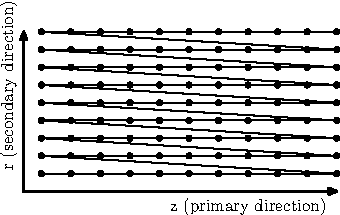
\includegraphics[origin=bl,height=40mm,angle=0]{./figures/Fieldmaps/order-1.pdf}
    \caption[Order of field values in a 2D field map in XZ orientation]{2D field map with primary direction corresponding to the longitudinal, secondary direction to the transverse direction}
    \label{fig:order1}
  \end{center}
\end{figure}

\begin{figure}[ht]
  \begin{center}
    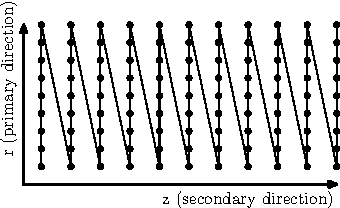
\includegraphics[origin=bl,height=40mm,angle=0]{./figures/Fieldmaps/order-2.pdf}
    \caption[Order of field values in a 2D field map in ZX orientation]{2D field map with primary direction corresponding to the transverse, secondary direction to the longitudinal direction}
    \label{fig:order2}
  \end{center}
\end{figure}

For the 2D dynamic case in XZ orientation there are four columns: $E_z$, $E_r$, an unused column and $H_t$ in this order. In the other orientation the first and the second column and the third and fourth column are interchanged.

On the second line of the header of a 1D, 2D or 3D T7 type of field map the beginning and the end of the electromagnetic field relative to the physical element in primary direction is written (in centimeters!). Also written on the second line is the number of {\bf mesh spacings}, corresponding to the {\bf number of grid points minus 1}. For the ASTRA compatible field maps this line is omitted.

On the third line is the frequency. For static cases this line is omitted. The frequency is on the second line of a AstraDynamic field map.

The fourth line corresponds to the second line but in secondary direction and the fifth accordingly for the tertiary direction. In the case of a 1D or 2D the fifth line is omitted since there is no tertiary direction. Those two lines are omitted in the ASTRA compatible field maps.

On the sixth line follows the first line with field values as described above.

Even though there is no secondary direction in the 1D case the header of a 1D field map is equal to its 2D equivalent: the elements can be provided with a boolean attribute FAST which has only an effect in conjunction with a 1D field map. The code then generates internally a 2D field map and the field strengths are interpolated as in the case of 2D and 3D field maps instead of being calculated using the Fourier coefficients. The fourth line determines the transverse dimension and the grain size of the produced mesh.

For examples of field maps see \appref{app_fieldmaps} on page~\pageref{chp:app_fieldmaps}.

The field maps {\bf 1DProfile1} and {\bf 1DProfile2} are different from the rest since no actual fields are stored but a profile. They are used to represent the fringe fields of various elements. The actual fields used in an \opalt simulation are calculated using Enge functions \cite{enge}. In turn, the Enge functions are declared in two different ways. A {\bf 1DProfile1} field map gives the coefficients of the Enge function explicitly. A {\bf 1DProfile2} field map stores the profile itself. From this profile the Enge coefficients are calculated by solving a least-square equation.

On the first line after the string describing the type of field map two integer numbers and a floating point number follow. The first integer number describes the number of Enge coefficients to be used for the entry fringe field, the second the equivalent for the exit fringe field. The floating point number specifies the full gap height. On the second line the first value describes the beginning of the entry fringe field (in local coordinates; corresponds to {\sl zbegin\_entry} in \figref{fringefields,fringefields-sbend}), the second the origin of the Enge polynomial, the third the end of the fringe field ({\sl zend\_entry}). The last number of this line is only used in {\bf 1DProfile2} and specifies the number of grid points minus 1 of the field profile. The third line looks identical to the sdcond, but the last value on this line is not used yet. The values on this line correspond to {\sl zbegin\_exit, origin of Enge function} and {\sl zend\_exit} in \figref{fringefields,fringefields-sbend}. The following lines are the coefficients of the Enge function in the case of {\bf 1DProfile1} and the actual field profile in {\bf 1DProfile2}, see \appref{app_fieldmaps}.

Note that {\sl zbegin\_entry}, {\sl zend\_entry}, {\sl zbegin\_exit} and {\sl zend\_exit} have slightly different definitions when defining a rectangular bend as opposed to a sector bend (\figref{fringefields,fringefields-sbend}).



\begin{figure}[ht]
  \begin{center}
    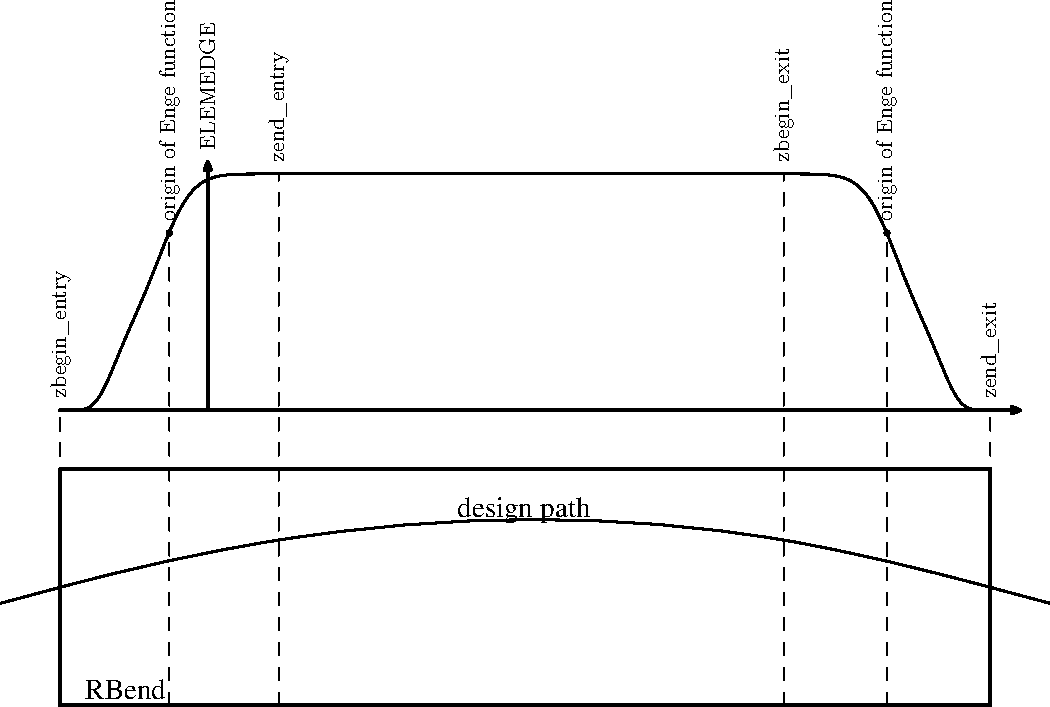
\includegraphics[origin=bl,height=100mm,angle=0]{./figures/Fieldmaps/profile-1.pdf}
    \caption{The profile of a rectangular bend and its corresponding design path.}
    \label{fig:fringefields}
  \end{center}
\end{figure}

\begin{figure}[ht]
  \begin{center}
   % 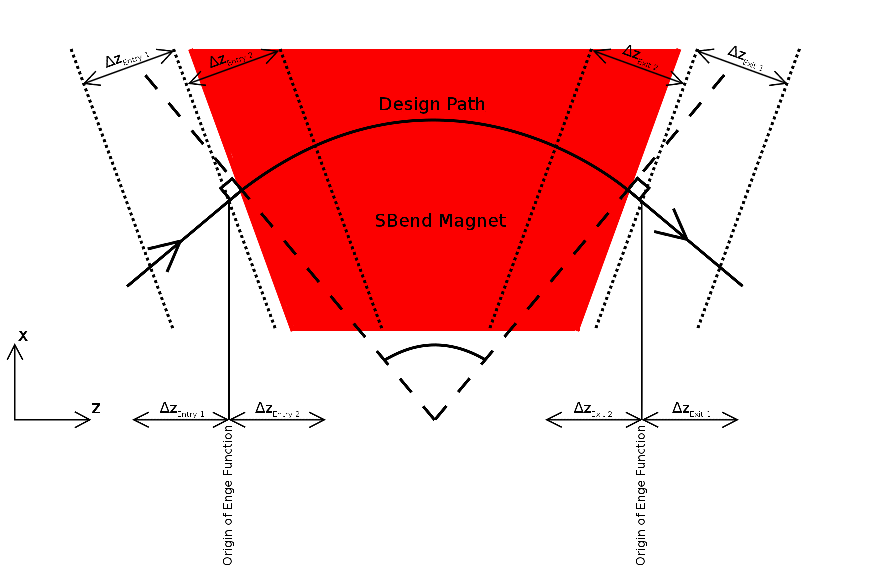
\includegraphics[origin=bl,height=100mm,angle=0]{./figures/Fieldmaps/profile-sbend.pdf}
   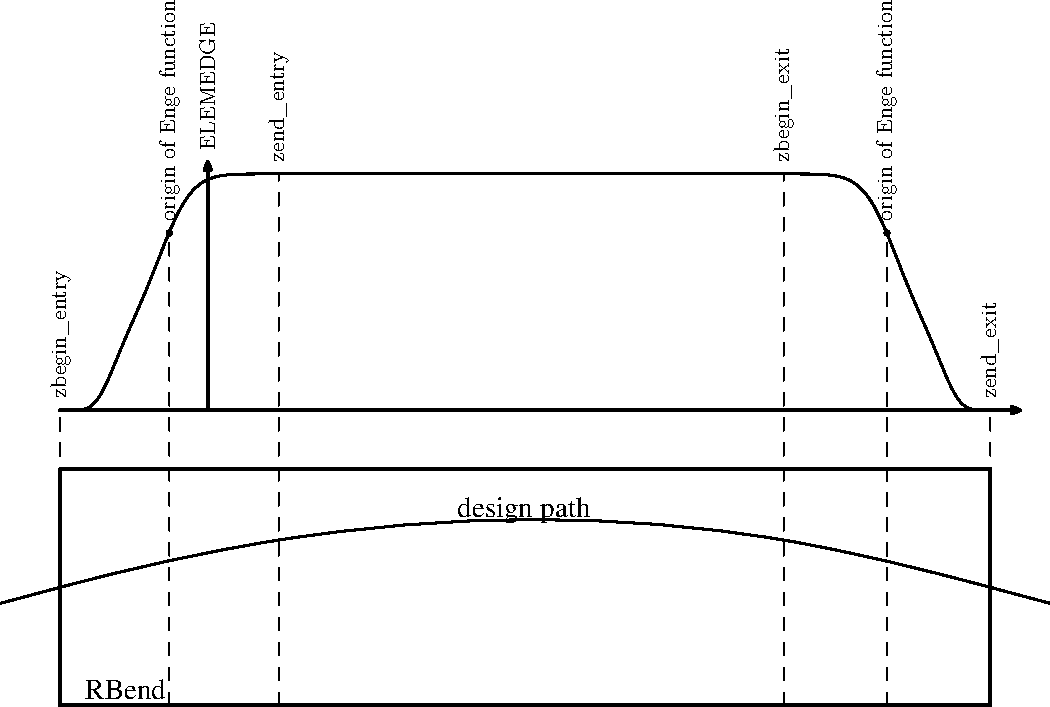
\includegraphics[origin=bl,height=100mm,angle=0]{./figures/Fieldmaps/profile-1.pdf}
    \caption{FIXME The location and definitions of the Enge function coefficients for a sector bend
      and its corresponding design path.}
    \label{fig:fringefields-sbend}
  \end{center}
\end{figure}

\clearpage

\leftpointright As a general warning: be wise when you choose the type of field map to be used! The following three pictures show the longitudinal phase space after three gun simulations using different types of field maps. In the first picture, \Figure{figure_1ddynamic_step82}, we used a 1D field map which stores a sampling of the electric field in longitudinal direction, $E_z$. From these values $E_z$, $E_r$ and $B_t$ off-axis are calculated resulting in a smooth field. All field maps we used are made of the same solution file from a Poisson/Superfish simulation.
\begin{figure}
  %
  \begin{center}
  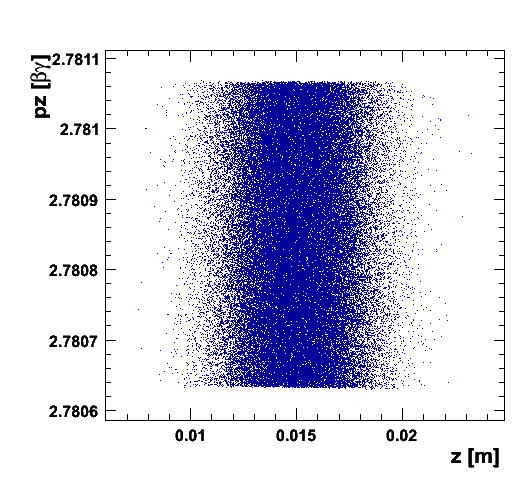
\includegraphics[origin=bl,height=80mm,angle=0]{./figures/Fieldmaps/1DDynamic_step82.png}
  %
  \caption{\label{fig:1ddynamic_step82}
    The longitudinal phase space after a gun simulation using a 1D field map (on-axis field) of the gun.
  }
  %
  \end{center}
%
\end{figure}

In \Figure{figure_1ddynamic_fast_step82} we used the same on-axis field map as in the first but we used the FAST switch which constructs a 2D field map from the on-axis field maps. Between the grid points the fields are calculated using a linear interpolation. Here we see a structure which can be influence using more grid points in transverse direction.
\begin{figure}
  %
  \begin{center}
  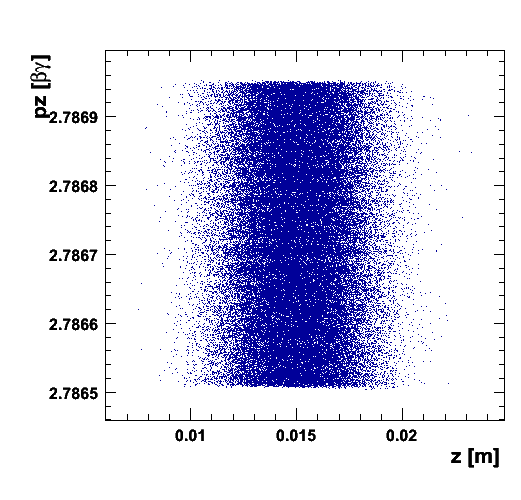
\includegraphics[origin=bl,height=80mm,angle=0]{./figures/Fieldmaps/1DDynamic_fast_step82.png}
  %
  \caption{\label{figure_1ddynamic_fast_step82}
    The longitudinal phase space after a gun simulation using a 1D field map (on-axis field) of the gun in combination with the FAST switch.
  }
  %
  \end{center}
%
\end{figure}
In the last picture, \Figure{figure_2ddynamic_step82}, we generated directely a 2D field map from the solution file of Poisson/Superfish. Here we could observe two different structures: first the fine structure stemming from the linear interpolation and secondly a much stronger structure of unknow origin.
\begin{figure}
  %
  \begin{center}
  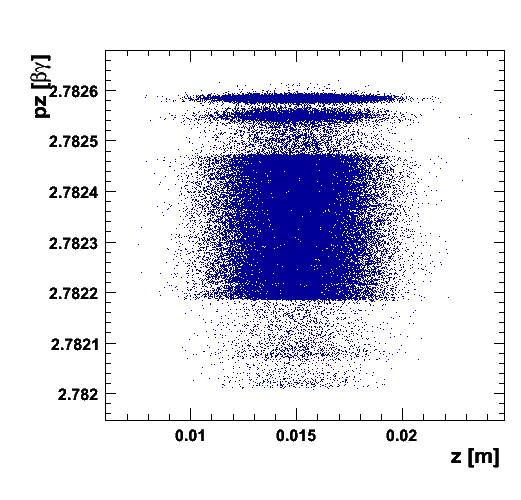
\includegraphics[origin=bl,height=80mm,angle=0]{./figures/Fieldmaps/2DDynamic_step82.png}
  %
  \caption{\label{figure_2ddynamic_step82}
    The longitudinal phase space after a gun simulation using a 2D field map of the gun generated by Poisson/Superfish.
  }
  %
  \end{center}
%
\end{figure}


\subsection{Field Maps from the Femaxx 3D Eigenmode Solver}

Electromagnetic field maps for beam dynamics calculations originate from a number of different
electromagnetic solvers, e.g. Superfish and similar codes.
%%
%%
Here, we describe the current status of work in progress which will, eventually,
allow the usage of field maps that have been computed with the femaxx $3$-dimensional
electromagnetic eigenmodal solver \cite{bib:arbenzetal2001,bib:arbenzetal2006}.
%%
%%
The femaxx code computes electromagnetic eigenmodes of resonant cavities of
arbitrary $3$-dimensional shape and boundary conditions.
%%
Unlike Superfish and similar $2$-dimensional codes, femaxx is not restricted in the
kind of geometry it can model. It is therefore possible to consider arbitrary
shapes and their inclusion in beam dynamics and particle tracking calculations.
%%
%%
Given a mesh of a $3$-dimensional geometry femaxx computes eigenomdal field
decompositions.
%%
The user then specifies sampling locations for the electromagnetic eigenfields.
%%
At present, sampling locations are specified in terms of a cylinder shape,
i.e. the user indicates the cylinder axis, the radial cylinder vector and
the number of sampling locations in axial, radial and azimuthal directions.
%%
Once the eigenmodal solution has been computed the fields are sampled at
these locations and stored in the T7 file format, for subsequent use in \opal.
%%
Considerable effort has been spent for the validation and benchmarking of
beam dynamics calculations based on T7 field maps computed with femaxx.
%%
A pillbox cavity, i.e. a cylinder shape with a radius $r = 4.7$cm and
height $h = 3$ cm, has been chosen for benchmarking purposes,
due to the availability of an analytical solution.
%%
The analytical resonance frequency of the dominant mode is $2.441$ GHz.
%%
%%
We have compared two cases with \opal: (1) The analytical solution has been
sampled within a cylinder volume, stored into a T7 file and used in an \opal
run; (2) the same pillbox shaped geometry has been discretization into tetrahedra
and the eigenmodal fields were calculated with femaxx.
%%
These two cases were then compared, resulting in the following conclusions:
%%
(1) Using a relatively coarse mesh with some $110'000$ tetrahedra, the difference
between the analytical and the numerical solution was usually smaller than
$1$ percent.
%%
(2) Using an adaptively refined mesh, the difference between analytical and
numerical solutions decreased below $1$ pro mille. The mesh is shown
in \figref{figure_pillbox_adaptively_refined_mesh}.
%%
(3) It is thereofore imperative to usa a tetrahedral mesh which has been
refined around the beam axis. It is definitely more efficient to use local
refinement, based on physical argument, than simply refine the complete
mesh in a uniform manner.
%%


We are now working towards benchmarking more complicated shapes in order to
assess requirements w.r.t to meshes and modeling geometry so that we
achieve the same or better accuracy as has been obtained from field
maps that were computed with Superfish like solvers based on azimuthal symmetry.

\begin{figure}
  %
  \begin{center}
  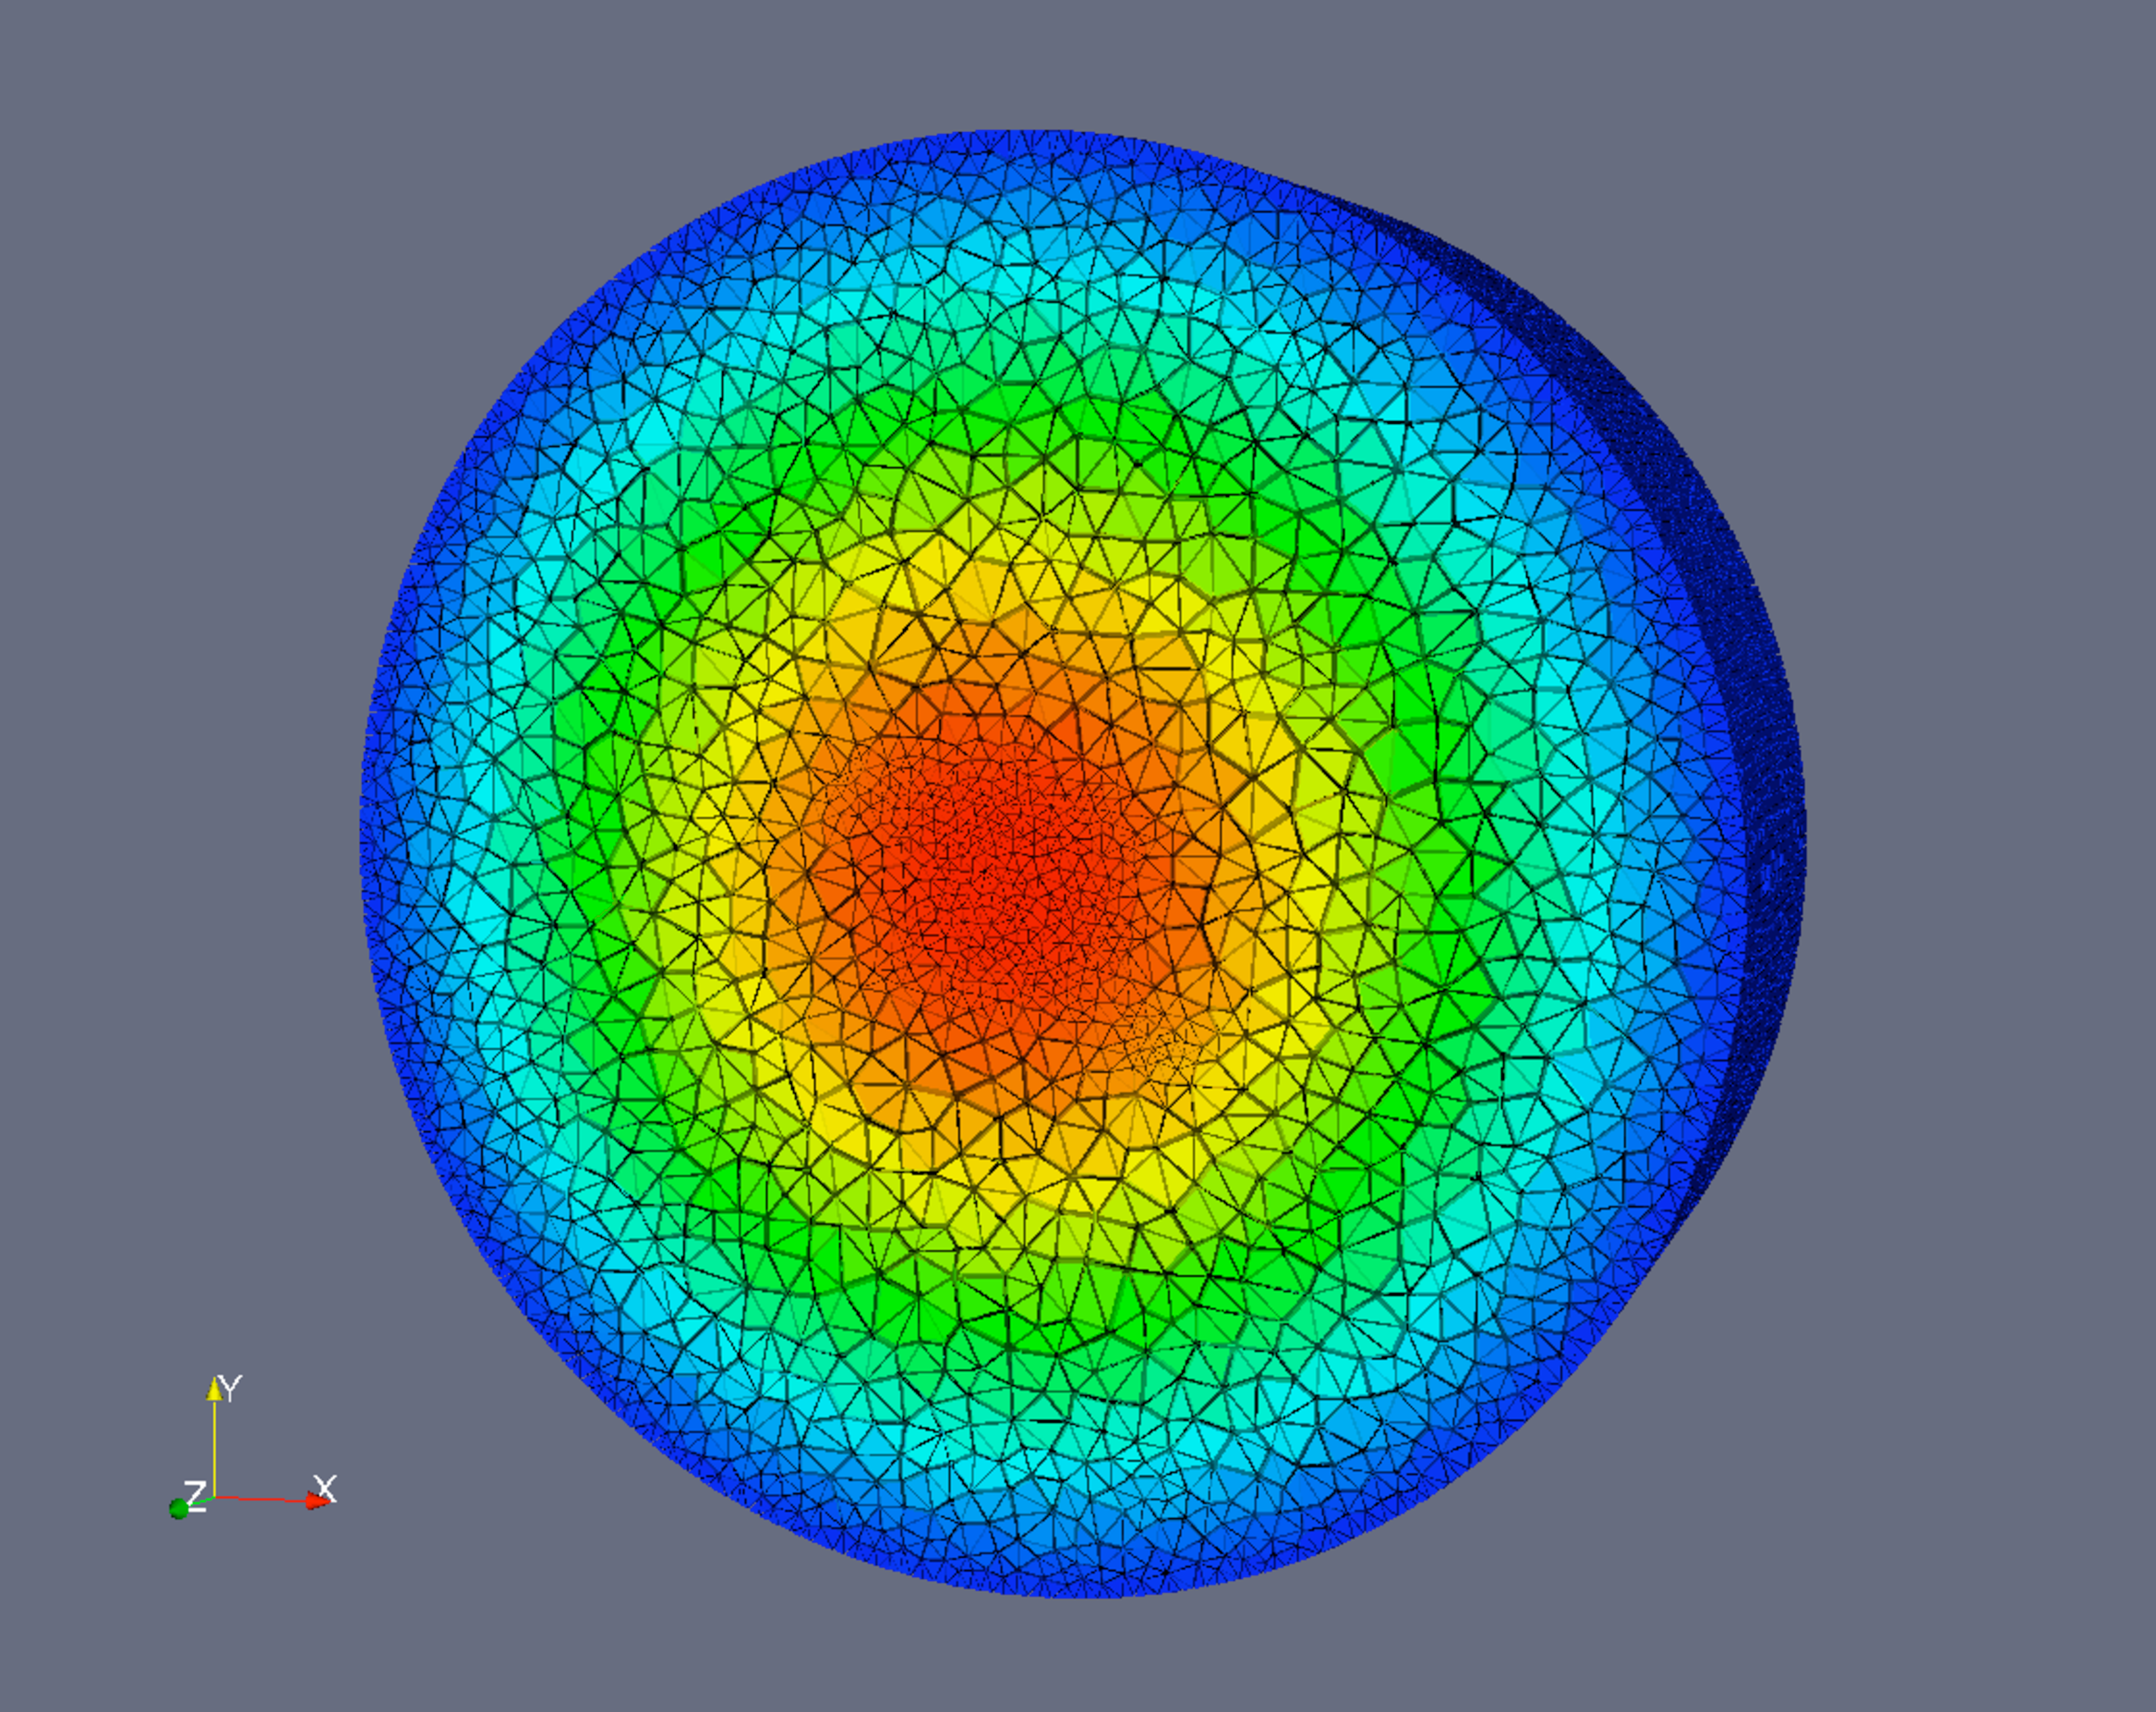
\includegraphics[origin=bl,width=80mm,angle=0]{./figures/adaptivePillboxMesh.pdf}
  %
  \caption[Tetrahedral mesh of a pillbox shaped cavity]{\label{figure_pillbox_adaptively_refined_mesh}
    We show the discretization of a pillbox shaped cavity geometry
        into a tetrahedral mesh. The mesh has been adaptively
        refined so that the region around the cylinder axis is
        decomposed into smaller tetrahedra than those which are
        further away from the axis.
  }
  %
  \end{center}
%
\end{figure}

\clearpage
\subsection{Output}
The data is stored in the H5hut file-format \cite{bib:howison2010} and can be analysed
using the H5root \cite{bib:schietinger}. The frequency
of the data output (phase space and some statistical quantities) can be set using the %FIXME {OPTION} statement \seesec{option},
statement and the flag PSDUMPFREQ. The file is named like in input file but the extension is {\tt .h5}.

\begin{figure}[ht]
 \begin{center}
 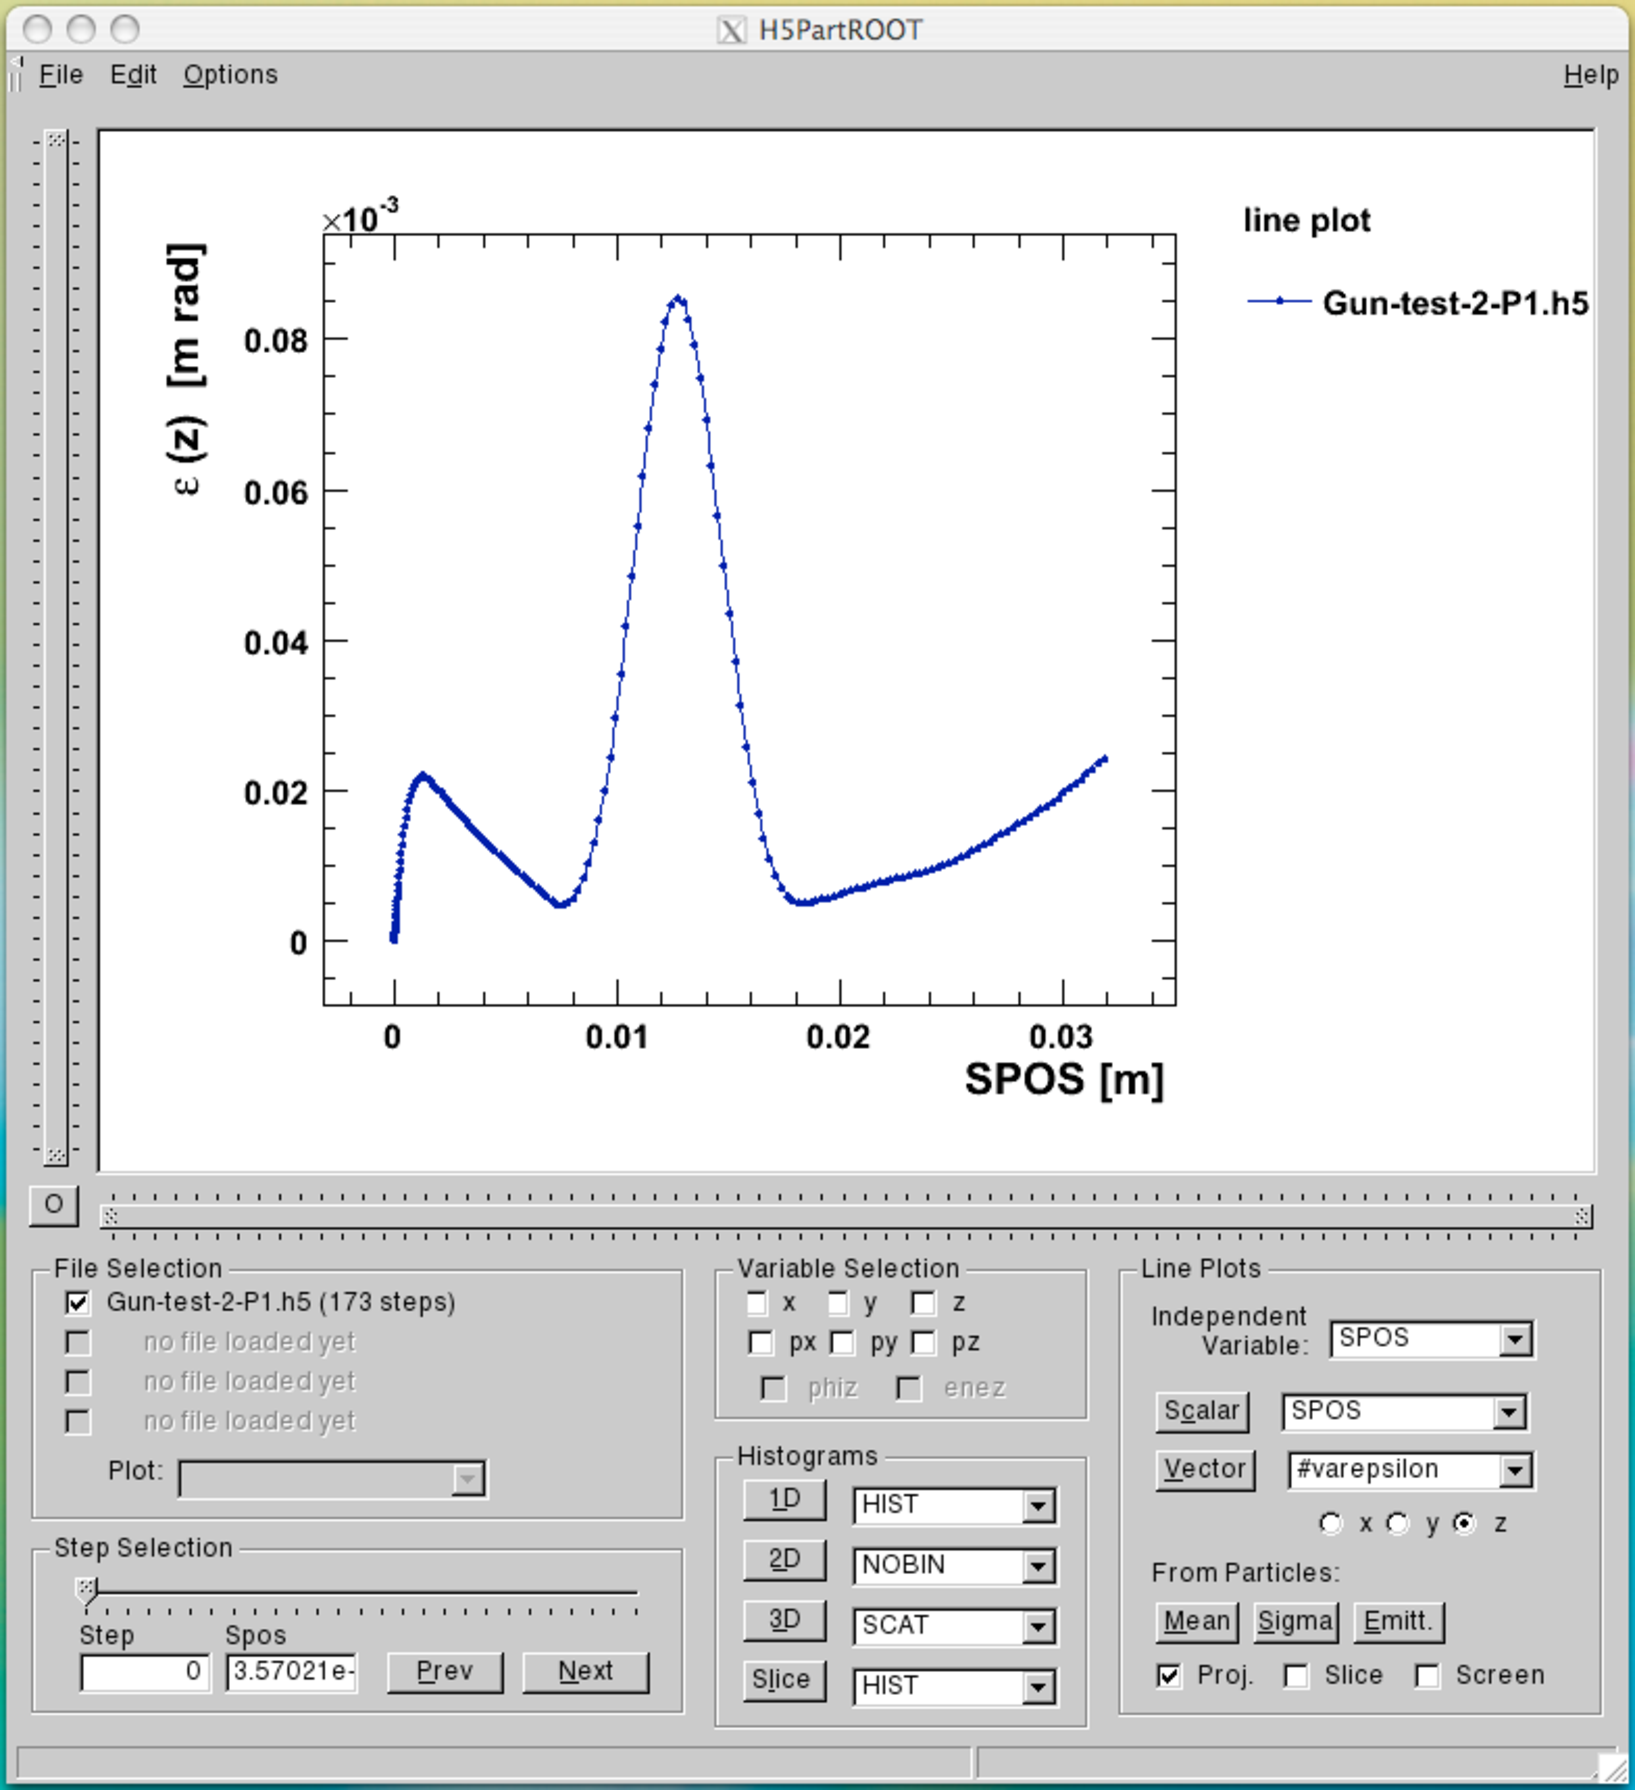
\includegraphics[width=0.45\linewidth,angle=0]{figures/H5rootPicture1}
  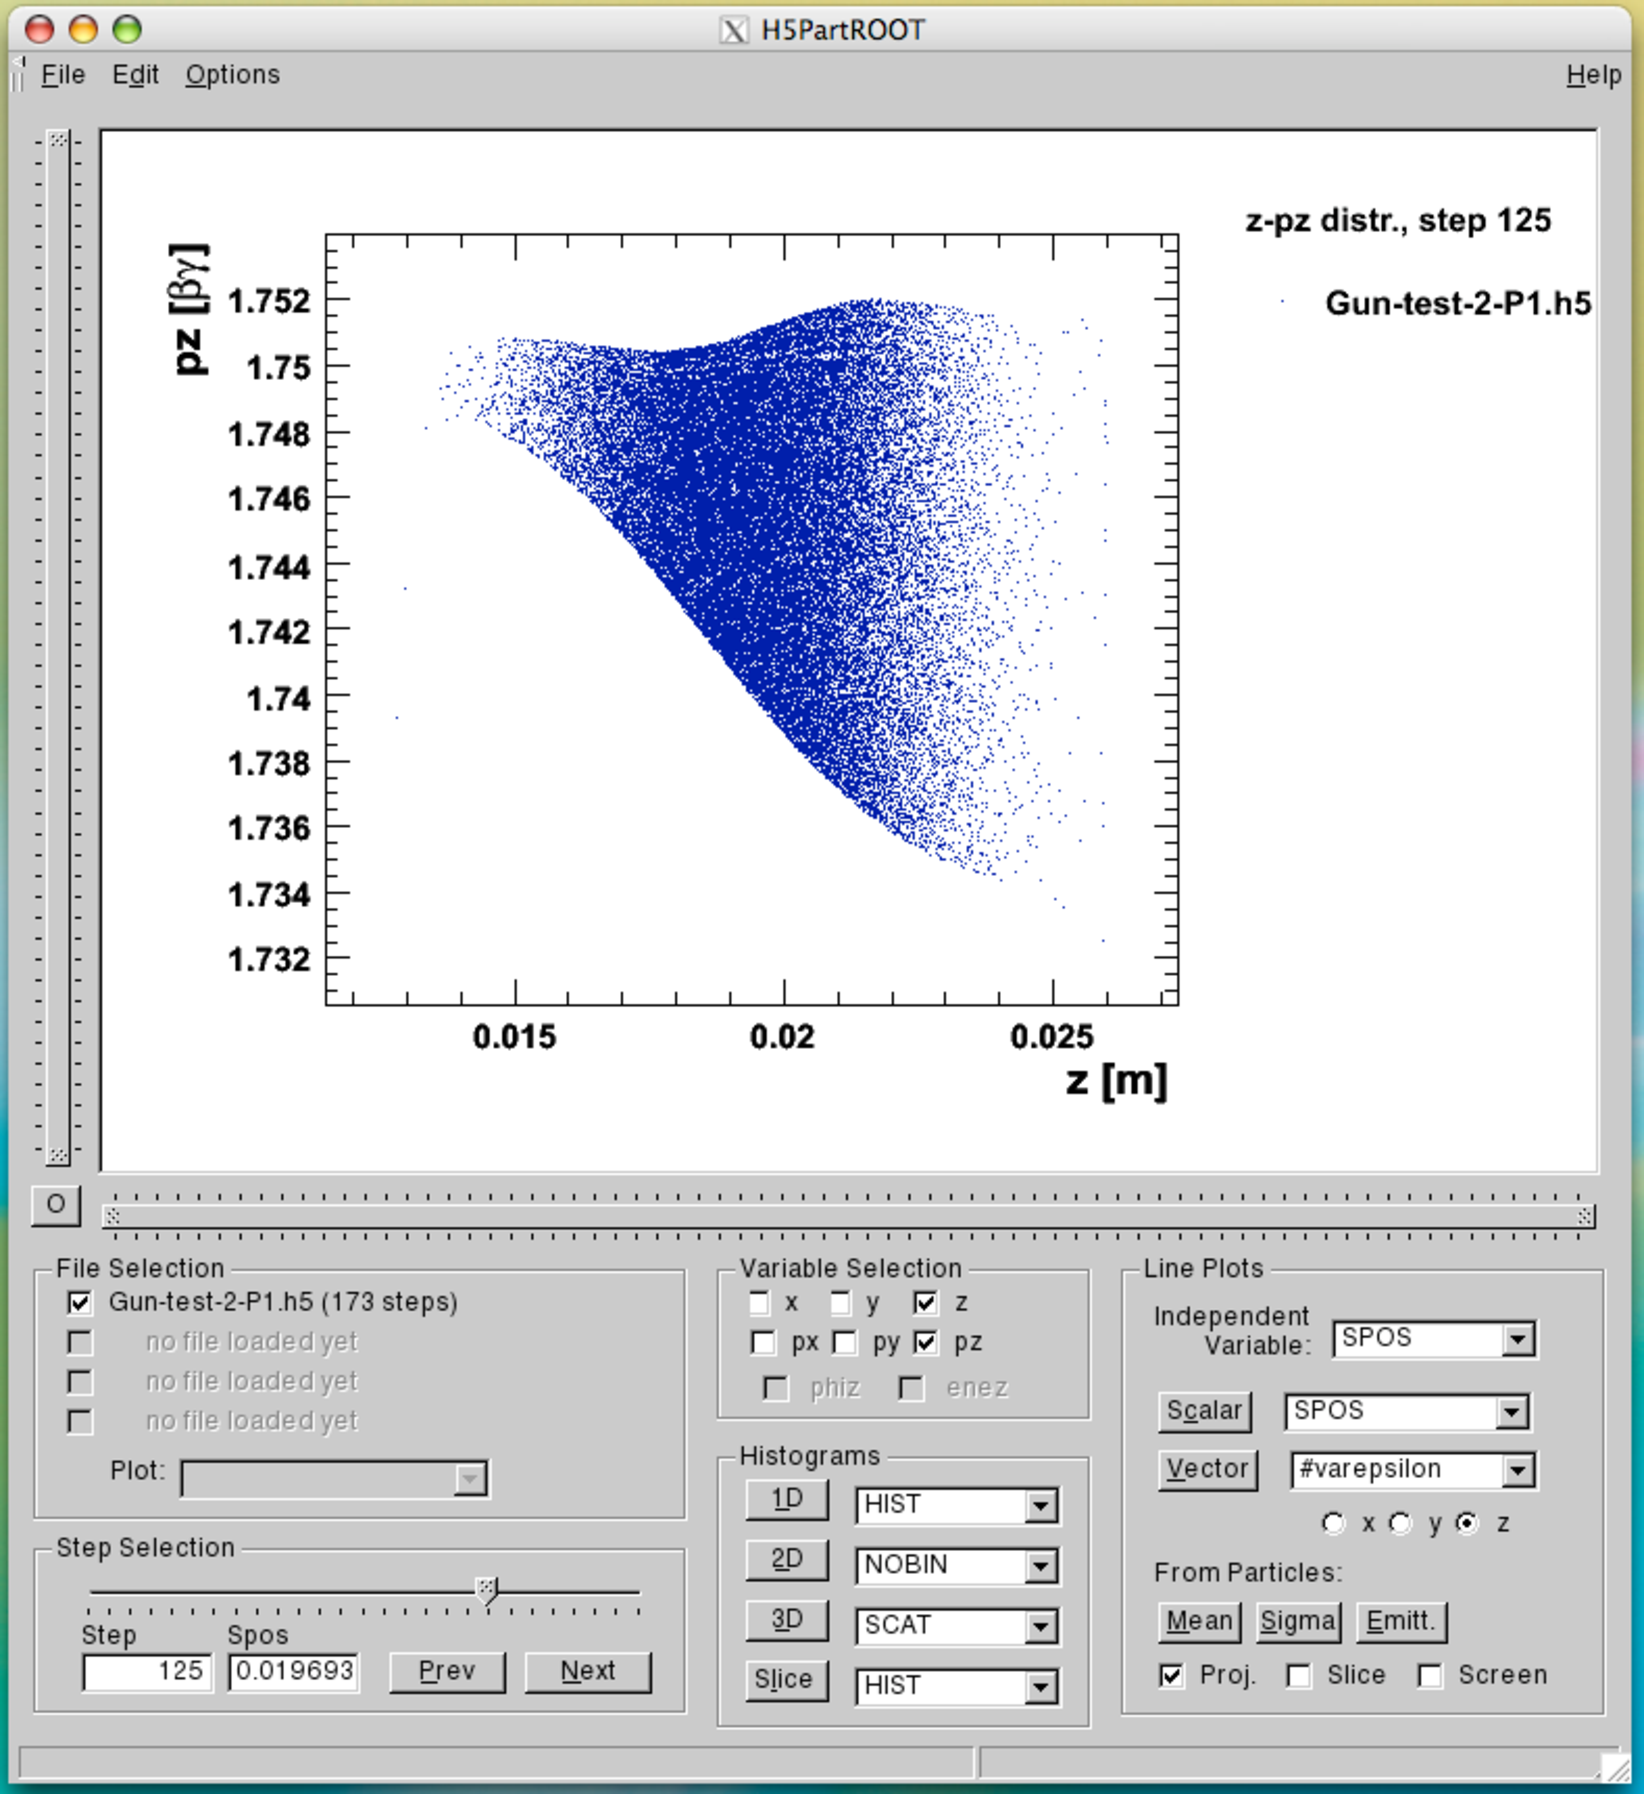
\includegraphics[width=0.45\linewidth,angle=0]{figures/H5rootPicture2}
  \caption{H5root enables a variety of data analysis and post processing task on \opal data}
  \label{fig:h5root1}
 \end{center}
\end{figure}



\begin{figure}[ht]
 \begin{center}
   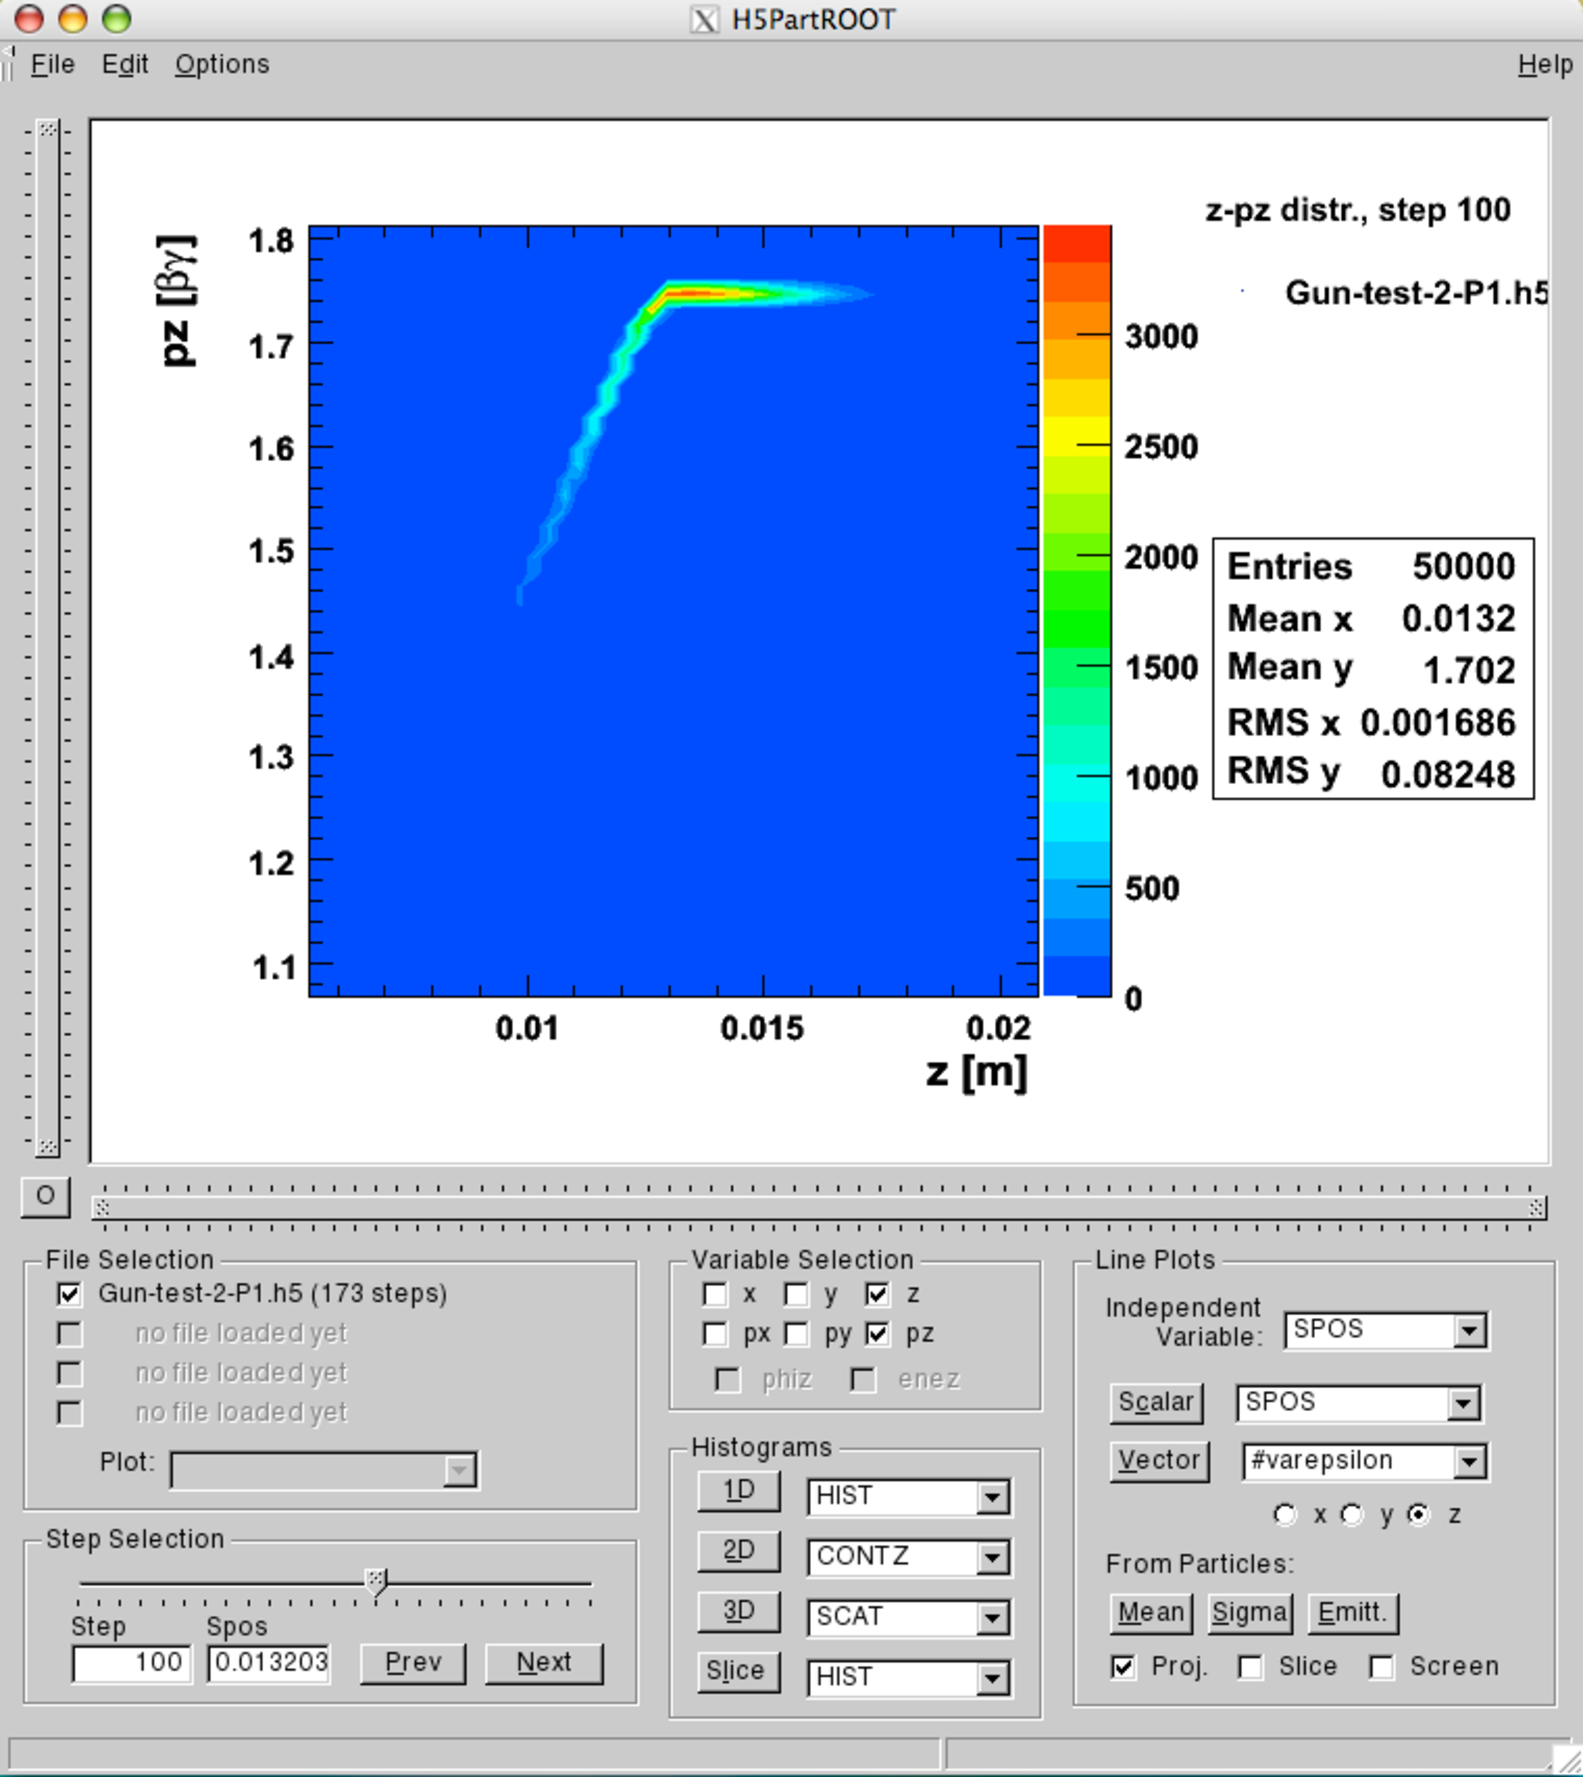
\includegraphics[width=.9\linewidth,angle=0]{figures/H5rootPicture3}
  \caption{Example of a longitudinal phase space shown with H5root}
  \label{fig:h5root2}
 \end{center}
\end{figure}



An ASCII file with statistical beam
parameters is stored in a {\tt .stat} file. An SDDS file output is in preparation.

\section{\opalcycl}
\label{sec:opalcycl}
\index{opalFlavours}

\subsection{Introduction}

\opalcycl is a fully three-dimensional parallel beam dynamics simulation program dedicated to future high intensity cyclotrons
which is capable of both doing single particle tracking for conventional beam dynamics designs and
multiple particles tracking which takes into account the space charge effects.

For the first time in the cyclotron community, \opalcycl has the capability to track multiple bunches simultaneously
and take into account the beam-beam effects of the radial neighboring bunches (we call it neighboring bunch effects for short)
by using a self-consistent numerical simulation model.

According to the number of particles defined (by the argument \texttt{NPART} in \texttt{BEAM}, see \chpref{beam}) ,
\opalcycl selects the following three operation modes automatically:

\begin{description}

\item[Single Particle Tracking mode]

  In this mode, only one particle is tracked, either with acceleration or not.  Working in this mode, \opalcycl
  can be used as a tool during the preliminary design phase of a cyclotron.

  The 6D parameters of a single particle in the initial local frame must be read from a file. To do this, in the \opal input file,
  the command line \texttt{DISTRIBUTION} \seechp{distribution} should be defined like this:
\begin{verbatim}
  Dist1: DISTRIBUTION, TYPE=fromfile,
         FNAME="PartDatabase.dat";
\end{verbatim}
 where the file $PartDatabase.dat$ should have two lines:
\begin{verbatim}
 1
 0.001 0.001   0.001   0.001   0.001  0.001
\end{verbatim}
The number in the first line is the total number of particles.
In the second line the data represents $x, p_x, y,$$ p_y, z, p_z$ with the reference particle
in the local frame. The units are described in \secref{variablesopalcycl}.

Please don't try to run this mode in parallel environment. You should believe that a single processor of the 21st century is capable of doing
the single particle tracking.

\item[Tune Calculation mode]

  In this mode, two particles are tracked, one with all data is set to zero is the reference particle and another one is an off-centering particle
  which has a little shift from the other one in both $r$ and $z$ directions. Working in this mode, \opalcycl can
  calculate the betatron oscillation frequency $\nu_r$ and $\nu_z$ for different energies to evaluate the focusing characteristics
  for a given magnetic field.

  Like the single particle tracking mode,
  the 6D parameters of the two particles in initial local frame must be read from a file, too.
  In the file should has three lines:
\begin{verbatim}
 2
 0.0   0.0   0.0   0.0   0.0   0.0
 0.001 0.0   0.0   0.0   0.001  0.0
\end{verbatim}

When the total particle number equals 2, this mode is triggered automatically.
Only the element \texttt{CYCLOTRON} in the beam line is used and other elements are omitted if any exists.

Please don't try to run this mode in parallel environment, either.


\item[Multi-particle tracking mode]

  In this mode, large scale particles can be tracked simultaneously, either with space charge or not,
  either single bunch or multi-bunches, either serial or parallel environment,
  either reading the initial distribution from a file or generating a typical distribution,
  either running from the beginning or restarting from the last step of a former simulation.

  Because this is the main mode as well as the key part of \opalcycl,
  we will describe this in detail in \secref{opalcycl:MultiBunch}.

\end{description}

Generally speaking, the following aspects may be considered for quantitatively studying high intensity beam dynamics in cyclotrons:
  \begin{itemize}
  \item large scale particles, as many as possible, which is of course limited by computer sources;
  \item measured magnetic field map or numerical calculated field with high precision;
  \item numerical integrator with high precision;
  \item powerful parallel Poisson solver with high precision and resolution;
  \item imperfection and misalignment of the machine;
  \item the influences of other factors induced by high intensity, such as beam-beam effects and weak field effects induced in the cavities.
  \end{itemize}
  In the following sections of this chapter, some of the above issues will be described in detail for \opalcycl.

\subsection{Field Map}
In \opalcycl, the magnetic field is read from an ASCII type file. The field data should be stored in the cylinder coordinates frame
( because the field map on the median plane of the cyclotron is usually measured in this frame ).

There are two possible situations. One is the real field map on median plane of the exist cyclotron machine using measurement equipment.
Limited by the narrow gaps of magnets, in most cases with cyclotrons, only vertical field $B_z$ on the median plane ($z=0$) is measured.
Since the magnetic field data off the median plane field components is necessary for those particles with $z \neq 0$, the field need to be expanded in $Z$ direction.
According to the approach given by Gordon and Taivassalo, by using a magnetic potential and measured $B_z$ on the median plane,
at the point $(r,\theta, z)$ in cylindrical polar coordinates, the 3$th$ order field can be written as
\begin{eqnarray}\label{eq:Bfield}
  B_r(r,\theta, z) & = & z\diffp{B_z}{r}-\frac{1}{6}z^3 C_r, \nonumber\\
  B_\theta(r,\theta, z) & = & \frac{z}{r}\diffp{B_z}{\theta}-\frac{1}{6}\frac{z^3}{r} C_{\theta}, \\
  B_z(r,\theta, z) & = & B_z-\frac{1}{2}z^2 C_z,  \nonumber
\end{eqnarray}
where $B_z\equiv B_z(r, \theta, 0)$ and
\begin{eqnarray}\label{eq:Bcoeff}
  C_r & = & \diffp[3]{B_z}{r} + \frac{1}{r}\diffp[2]{B_z}{r} - \frac{1}{r^2}\diffp{B_z}{r}
        + \frac{1}{r^2}\diffp{B_z}{{r}{\theta^2}} - 2\frac{1}{r^3}\diffp[2]{B_z}{\theta}, \nonumber  \\
  C_{\theta} & = & \frac{1}{r}\diffp{B_z}{{r}{\theta}} + \diffp{B_z}{{r^2}{\theta}}
        + \frac{1}{r^2}\diffp[3]{B_z}{\theta},  \\
  C_z & = & \frac{1}{r}\diffp{B_z}{r} + \diffp[2]{B_z}{r} + \frac{1}{r^2}\diffp[2]{B_z}{\theta}. \nonumber
\end{eqnarray}

All the partial differential coefficients are on the median plane and can be calculated by interpolation. \opalcycl uses  Lagrange's  5-point formula.

The other situation is to calculate the field on the median plane or the 3D fields of the working gap for interesting region numerically by creating 3D model using commercial software,
such as TOSCA, ANSOFT and ANSYS during the design phase of a new machine. If the field on the median plane is calculated, the field off the median plane can be obtained using
the same expansion approach as the measured field map as described above. However, the 3D fields of the entire working gap should be more accurate than
the expansion approach  especially at the region not so close to the median plane in $Z$ direction.

In the current version, we implemented the three specific type field-read functions $Cyclotron::$$getFieldFromFile()$ of the median plane fields.
That which function is used is controlled by the parameters TYPE of CYCLOTRON \seesec{cyclotron} in the input file.
\begin{enumerate}
\item TYPE=CARBONCYCL.
Program reads in the median plane field date $B_z$ (in kGauss) from a file in which the data is arranged as shown in \figref{CYCLField}.
This function is originally for the field map of the PSI 450 MeV C12 cyclotron which is under design but can serve as a simple way to import ASCII
field maps.
\begin{figure}[ht]
  \begin{center}
    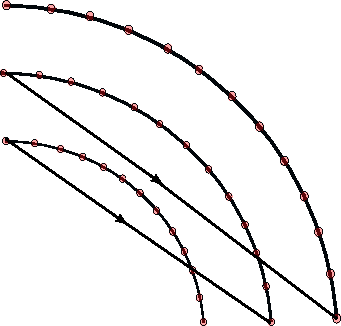
\includegraphics[origin=bl,height=40mm]{./figures/cyclotron/CarbonFieldFormat.pdf}
    \caption{2D field map on the median plane with primary direction corresponding to the azimuthal direction, secondary direction to the radial direction}
    \label{fig:CYCLField}
  \end{center}
\end{figure}
We need to add 6 parameters at the header of a plain $B_z$ (kGauss) data file, namely,
$r_{min}$ [mm], $\Delta r$ [mm], $\theta_{min}$[$^\circ$], $\Delta \theta$[$^\circ$],
$N_\theta$ (total data number in each arc path of azimuthal direction) and $N_r$ (total path number along radial direction).
If $\Delta r$ or $\Delta \theta$ is decimal, one can set its negative opposite number. For instance, if $\Delta \theta = \frac{1}{3}^\circ$, the fourth line of the header should be set to -3.0.
Example showing the above explained format:
\begin{fmpage}
\begin{footnotesize}
\begin{verbatim}
3.0e+03
10.0
0.0
-3.0
300
161
1.414e-03  3.743e-03  8.517e-03  1.221e-02  2.296e-02
3.884e-02  5.999e-02  8.580e-02  1.150e-01  1.461e-01
1.779e-01  2.090e-01  2.392e-01  2.682e-01  2.964e-01
3.245e-01  3.534e-01  3.843e-01  4.184e-01  4.573e-01
                        ......
\end{verbatim}
\end{footnotesize}
\end{fmpage}
\item TYPE=CYCIAE.

Program reads in the median plane fields $B_z$ calculated by ANSYS\,10.0.  This function is originally for the 100 MeV cyclotron of CIAE,
 whose isochronous fields is numerically computed by by ANSYS. The median plane fields data is output by reading the APDL (ANSYS Parametric Design Language) script
during the post-processing phase (you may need to do minor changes to adapt your own cyclotron model):
\begin{fmpage}
\begin{footnotesize}
\begin{verbatim}
/post1
resume,solu,db
csys,1
nsel,s,loc,x,0
nsel,r,loc,y,0
nsel,r,loc,z,0
PRNSOL,B,COMP

CSYS,1
rsys,1

*do,count,0,200
   path,cyc100_Ansys,2,5,45
   ppath,1,,0.01*count,0,,1
   ppath,2,,0.01*count/sqrt(2),0.01*count/sqrt(2),,1

   pdef,bz,b,z
   paget,data,table

   *if,count,eq,0,then
      /output,cyc100_ANSYS,dat
      *STATUS,data,,,5,5
      /output
   *else
      /output,cyc100_ANSYS,dat,,append
      *STATUS,data,,,5,5
      /output
   *endif
*enddo
finish
\end{verbatim}
\end{footnotesize}
\end{fmpage}
By run this in ANSYS, you can get a fields file with the name $cyc100\_ANSYS.data$.
You need to  put 6 parameters at the header of the file, namely,
$r_{min}$ [mm], $\Delta r$ [mm], $\theta_{min}$[$^\circ$], $\Delta \theta$[$^\circ$],
$N_\theta$(total data number in each arc path of azimuthal direction) and $N_r$(total path number along radial direction).
If $\Delta r$ or $\Delta \theta$ is decimal,one can set its negative opposite number. This is useful is the decimal is unlimited.
For instance,if $\Delta \theta = \frac{1}{3}^\circ$, the fourth line of the header should be -3.0.
In a word, the fields are stored in the following format:
\begin{fmpage}
\begin{footnotesize}
\begin{verbatim}
0.0
10.0
0.0e+00
1.0e+00
90
201
 PARAMETER STATUS- DATA  ( 336 PARAMETERS DEFINED)
                  (INCLUDING    17 INTERNAL PARAMETERS)

      LOCATION                VALUE
        1       5       1   0.537657876
        2       5       1   0.538079473
        3       5       1   0.539086731
                  ......
       44       5       1   0.760777286
       45       5       1   0.760918663
       46       5       1   0.760969074

 PARAMETER STATUS- DATA  ( 336 PARAMETERS DEFINED)
                  (INCLUDING    17 INTERNAL PARAMETERS)

      LOCATION                VALUE
        1       5       1   0.704927299
        2       5       1   0.705050993
        3       5       1   0.705341275
                  ......
\end{verbatim}
\end{footnotesize}
\end{fmpage}


\item If the value of TYPE is other string rather than above two, programme read in field data from the PSI format field file {\small{ZYKL9Z.NAR}} and {\small{SO3AV.NAR}}.
We add 4 parameters at the header of the file, namely,
$r_{min}$ [mm], $\Delta r$ [mm], $\theta_{min}$[$^\circ$], $\Delta \theta$[$^\circ$],
This is the default function for reading fields data.
If $\Delta r$ or $\Delta \theta$ is decimal,one can set its negative opposite number. This is useful is the decimal is unlimited.
For instance,if $\Delta \theta = \frac{1}{3}^\circ$, the fourth line of the header should be -3.0.
\end{enumerate}
{\bfseries You should revise the function or write your own function according to the instructions in the code to match your own field
format if it is different to above three types.}
The generic interface function for both the 2D measured map and the 3D field from file will be available in a later version.\\

For more detail about the parameters of CYCLOTRON, please refer to \secref{cyclotron}.

In the current version of \opalcycl, the RF cavities are treated as straight lines with infinitely narrow gaps
and the electric field is a $\delta$ function plus a transit time correction.
the two-gap cavity is treated as two independent single-gap cavities. the spiral gap cavity is not implemented yet.

For more detail about the parameters of cyclotron cavities, see \secref{cavity-cycl}.

The voltage profile of a cavity gap  is read from ASCII file. Here is an example:
\begin{verbatim}
6
0.00      0.15      2.40
0.20      0.65      2.41
0.40      0.98      0.66
0.60      0.88     -1.59
0.80      0.43     -2.65
1.00     -0.05     -1.71
\end{verbatim}
The number in the first line means 6 sample points and in the following lines the three values represent the normalized distance to
the inner edge of the cavity, the normalized voltage and its derivative respectively.

\subsection{Particle Tracking and Accelerating}

The precision of the tracking methods is vital for the entire simulation process, especially for long distance tracking jobs.
\opalcycl uses a 4th order Runge-Kutta algorithm and the second order Leap-Frog scheme. The 4th order Runge-Kutta algorithm needs 4 the external magnetic field evaluation in each time step $\tau$ .
During the field interpolation process, for an arbitrary given point the code first interpolates Formula $B_z$
for its counterpart on the median plane and then expands to this give point using \Eq{eq:Bfield}.

After each time step $i$, the code detects whether the particle crosses any one of the RF cavities during this step.
If it does, the time point $t_c$ of crossing is calculated and the particle return back to the start point of
step $i$. Then this step is divided into three substeps:
first, the code tracks this particle for $ t_1 = \tau - (t_c-t_{i-1})$;
then it calculates the voltage and adds momentum kick to the particle and refreshes its relativistic parameters $\beta$ and $\gamma$;
and then trackes it for $t_2 = \tau - t_1$.

\subsection{Space Charge Effects}

\opalcycl uses the same solvers as \opalt to calculate the space charge effects \seesec{opalFlavours:spacecharge}.
The difference is that, in a cyclotron,
both the origin and orientation of the local Cartesian frame are changed from time to time. So the coordinates are transformed from
the global frame to the local frame first, then the space charge fields are calculated in the local frame.
After the space charge fields are solved, both coordinates and self electric and magnetic field are transformed back to global frame.

In the current version, the space charge fields are calculated once for each time step and is kept constant during this step.

\subsection{Multi-bunches Issues}
\label{sec:opalcycl:MultiBunch}

The neighboring bunches problem is motivated by the fact that for high intensity cyclotrons with small turn
separation, single bunch space charge effects are not the only contribution. Along with the increment of beam
current, the mutual interaction of neighboring bunches in radial direction becomes more and more important,
especially at large radius where the distances between neighboring bunches get increasingly small and even they
can overlap each other. One good example is PSI 590 MeV Ring cyclotron with a current of about 2mA in
CW operation and the beam power amounts to 1.2 MW. A upgrade project for Ring is in process with
the goal of 1.8 MW CW on target by replacing four old aluminum resonators by four new copper cavities with peak
voltage increasing from about 0.7 MV to above 0.9 MV. After upgrade, the total turn
number is reduced from 200 turns to less then 170 turns.
Turn separation is increased a little bit, but still are at the same order
of magnitude as the radial size of the bunches. Hence once the beam current increases from 2 mA to 3 mA, the mutual space
charge effects between radially neighboring bunches can have significant impact on beam dynamics.
In consequence, it is important to cover neighboring bunch effects in the simulation to quantitatively study its impact on the beam dynamics.

In \opalcycl, we developed a new fully consistent algorithm of multi-bunches simulation.  We implemented two working modes, namely ,
\texttt{AUTO} and \texttt{FORCE}. In the first mode, only a single bunch is tracked and accelerated at the beginning,
until the radial neighboring bunch effects become an important factor to the bunches' beheaver. Then the new bunches will be injected automatically to
take these effects into accout. In this way, we can save time and memory sufficiently, and more important,
we can get higher precision for the simulation in the region where neighboring bunch effects are neglectable.
In the other mode, multi-bunches simulation starts from the injection points. This mode is appropriate for the machines in which this effects is
unneglectable since the injection point.

In the space charge calculation for multi-bunches, the computation region covers all bunches.
Because the energy of the bunches is quite different, it is inappropriate to use only one particle rest frame and a single Lorentz transformation any more.
So the particles are grouped into different energy bins and in each bin the energy spread is relatively small. We apply Lorentz transforming, calculate
the space charge fields and apply the back Lorentz transforming for each bin separately. Then add the field data together. Each particle has a ID number to identify
which energy bin it belongs to.

\subsection{Input}
All the three working modes of \opalcycl use an input file written in \mad language which will be described in detail in the following chapters.

For the  {\bfseries Tune Calculation mode}, one additional auxiliary file with the following format is needed.
\begin{verbatim}
   72.000 2131.4   -0.240
   74.000 2155.1   -0.296
   76.000 2179.7   -0.319
   78.000 2204.7   -0.309
   80.000 2229.6   -0.264
   82.000 2254.0   -0.166
   84.000 2278.0    0.025
\end{verbatim}
In each line the three values represent energy $E$, radius $r$ and $P_r$ for the SEO (Static Equilibrium Orbit)
at starting point respectively and their units are {\tt MeV,  mm,  mrad}.

A bash script $tuning.sh$ is shown on the next page, to execute \opalcycl for tune calculations.
\begin{fmpage}
\begin{footnotesize}
\begin{verbatim}
  #!/bin/bash
  rm -rf tempfile
  rm -f plotdata
  rm -f tuningresult

  exec 6<FIXPO_SEO
  N="260"
  j="1"
  while read -u 6 E1 r  pr
  # read in Energy, initil R and intial Pr of each
  # SEO from FIXPO output
  do
  rm -rf tempfile
  echo -n j =
  echo "$j"
  echo -n energy= > tempfile
  echo -n "$E1"  >> tempfile
  echo  ";" >> tempfile

  echo -n r=  >> tempfile
  echo -n "$r" >> tempfile
  echo ";" >> tempfile

  echo -n pr= >> tempfile
  echo -n "$pr" >> tempfile
  echo  ";" >> tempfile
  # execute OPAL to calculate tuning frquency and store
  opal testcycl.in --commlib mpi --info 0 | \
     grep "Max" >>tuningresult
  j=$[$j+1]
  done
  exec 6<&-
  rm -rf tempfile

  # post porcess
  exec 8<tuningresult
    rm -f plotdata
  i="0"

  while [ $i -lt $N ]
  do
  read -u 8 a b ur1 d
  read -u 8 aa bb uz1 dd
  echo "$ur1   $uz1" >>plotdata
  i=$[$i+1]
  done

  exec 8<&-
  rm -f tuningresult
\end{verbatim}
\end{footnotesize}
\end{fmpage}
To start execution, just run $tuning.sh$ which uses the input file $testcycl.in$ and the auxiliary file {\footnotesize$FIXPO\_SEO$}.
The output file is $plotdata$ from which one can plot the tune diagram.

\subsection{Output}
{\bfseries Single Particle Tracking mode}

The intermediate phase space data is stored in an ASCII file which can be used to
the plot the orbit. The file's name is combined by input file name (without extension) and  $-trackOrbit.dat$.
The data are stored in the global Cartesian coordinates.
The frequency of the data output can be set using the %FIXME {OPTION} statement \seesec{option} and the flag SPTDUMPFREQ.

The phase space data per STEPSPERTURN (a parameter in the TRACK command) steps is stored in an ASCII file.
The file's name is a combination of input file name (without extension) and $-after$$EachTurn.dat$.
The data is stored in the global cylindrical coordinate system.
Please note that if the field map is ideally isochronous, the reference particle of a given energy take exactly one revolution in STEPPERTURN steps;
Otherwise,the particle may not go through a full $360^\circ$ in STEPPERTURN steps.

There are 3 ASCII files which store the phase space data around $0$, $\pi/8$ and $\pi/4$ azimuths.
Their names are the combinations of input file name (without extension) and $-Angle0.dat$, $-Angle1.dat$ and $-Angle2.dat$ respectively.
The data is stored in the global cylindrical coordinate system, which can be used to check the property of the closed orbit.\\

{\bfseries Tune calculation mode}

 The tunes $\nu_r$ and $\nu_z$ of each energy are stored in a ASCII file with name $tuningresult$.\\

{\bfseries Multi-particle tracking mode}

The intermediate phase space data of all particles and some interesting parameters,
including RMS envelop size, RMS emittance, external field, time, energy, length of path, number of bunches and
tracking step, are stored in the H5hut file-format \cite{bib:howison2010} and can be analyzed
using the H5root \cite{bib:schietinger}.
The frequency of the data output can be set using the %FIXME {OPTION} statement \seesec{option} and the flag PSDUMPFREQ.
The file is named like the input file but the extension is $.h5$.

The intermediate phase space data of centeral particle (with ID of 0) and an off-centering particle (with ID of 1)
are stored in an ASCII file. The file's name is combined by the input file name (without extension) and $-trackOrbit.dat$.
The frequency of the data output can be set using the  %FIXME{OPTION} statement \seesec{option} and the flag SPTDUMPFREQ.


\ifthenelse{\boolean{ShowMap}}{
\section{\opalmap} \label{sec:SplitOperatorMethods}

Typically, the total Hamiltonian can be written as the sum of two parts, $H = H_{1} + H_{2}$,
which correspond to the external and space charge contributions respectively.
Such a situation is ideally suited to multi-map
symplectic Split-Operator methods~\cite{forestall}, also known as fractional step methods \cite{SanzSerna}.
A second-order accurate algorithm for a single step is given by
\begin{equation} \label{eq:splitOper1}
{\cal M}(\tau)={\cal M}_1(\tau/2)~{\cal M}_2(\tau)~{\cal M}_1(\tau/2) + \mathcal{O}(\tau^3)
\end{equation}
where $\tau$ denotes the step size, ${\cal M}_1$ is the map corresponding
%\eqref{eq:mad9pham}
to $H_{1}$  and ${\cal M}_2$ is the map corresponding to $H_{2}$.
If desired this approach can be
easily generalized to higher order accuracy using Yoshida's
scheme. % ~\cite{yoshida}.
This is the simplest 2nd order symplectic\footnote{Products of symplectic operators are symplectic as well.} Split-Operator integration method, which first applies all external forces for the first half of one integration step, then adds the complete influence of the internal forces for one entire integration step, and then applies another half of an integration step worth of external forces.
Details following when \opalmap is implemented.
}{}




\section{General Output}
\subsection{Timing Information}


\index{opalFlavours)}


%----------- Footer control ------------------
\ifthenelse{\boolean{FullOPALManual}}
{
  %do nothing
}
% else (for individual document creation)
{
\appendix
\printbibliography
\end{document}
}
%---------------------------------------------
